\documentclass{ndjflart}
%%% HIGHLY RECOMMENDED PACKAGES AND SETTINGS
%\usepackage{pdfsync}  %% if you know what this is use it or not.
\usepackage[T1]{fontenc}
%%%%%%%%%%%%%%%%%%%%%%%%%%%%%%
%% If your tex system is less than 2 years old (in 2012) the following
%% font options are available. If not comment them out.
\usepackage{tgtermes}
%       otherwise use alternative journal fonts
%\renewcommand{\rmdefault}{ptm} % system default Times font
\usepackage{mathptmx}
%%%     additional fonts
\usepackage[scaled=.92]{helvet}
%\setoptfont{enc={T1},fam={pop}} % if You have Optima font, uncomment this line
%%% MATH
\usepackage{amsthm,amsmath,amssymb}
\usepackage{mathrsfs}
%%% BIBLIOGRAPHY
\usepackage[numbers]{natbib}  %% numbers is required.
%%% LINKS
\usepackage[colorlinks,citecolor=blue,urlcolor=blue]{hyperref}  %%check

\usepackage{enumerate}

\artstatus{am} %%% leave this alone!!  That means you, too!!
%%%%%%%%theorems%%%%%
\usepackage{graphicx}
\usepackage{caption}
\usepackage{subcaption}

\theoremstyle{plain}
\newtheorem{conjecture}{Conjecture}[section]
\newtheorem{theorem}[conjecture]{Theorem}
\newtheorem{lemma}[conjecture]{Lemma}
\newtheorem{proposition}[conjecture]{Proposition}
\newtheorem{corollary}[conjecture]{Corollary}

\theoremstyle{definition}
\newtheorem{definition}[conjecture]{Definition}
\newtheorem{remark}[conjecture]{Remark}
\newtheorem{question}[conjecture]{Question}
\newtheorem{example}[conjecture]{Example}
\newtheorem{examples}[conjecture]{Examples}
\newtheorem{construction}[conjecture]{Construction}

\numberwithin{equation}{section}

\startlocaldefs

\DeclareMathOperator{\FO}{FO}
\DeclareMathOperator{\inv}{inv}
\DeclareMathOperator{\qr}{qr}
\DeclareMathOperator{\hlr}{hlr}
\DeclareMathOperator{\lr}{lr}
\DeclareMathOperator{\Cnt}{Cnt}
\DeclareMathOperator{\BIT}{BIT}
\DeclareMathOperator{\MSO}{MSO}
\DeclareMathOperator{\BNDP}{BNDP}
\DeclareMathOperator{\PG}{PG}
\DeclareMathOperator{\dom}{dom}
\DeclareMathOperator{\ran}{ran}
\DeclareMathOperator{\Fun}{Fun}
\DeclareMathOperator{\DetTrCl}{DetTrCl}
\DeclareMathOperator{\dtrcl}{dtrcl}
\DeclareMathOperator{\TrCl}{TrCl}
\DeclareMathOperator{\trcl}{trcl}
\DeclareMathOperator{\LFP}{LFP}
\DeclareMathOperator{\lfp}{lfp}
\DeclareMathOperator{\REACH}{REACH}
\DeclareMathOperator{\emb}{emb}
\DeclareMathOperator{\sub}{sub}
\DeclareMathOperator{\Inj}{inj}
\DeclareMathOperator{\bij}{bij}
\DeclareMathOperator{\Th}{Th}
\DeclareMathOperator{\elem}{elem}
\DeclareMathOperator{\cf}{cf}
\DeclareMathOperator{\cl}{cl}
\DeclareMathOperator{\Str}{Str}
\DeclareMathOperator{\Card}{Card}
\DeclareMathOperator{\ar}{ar}
\DeclareMathOperator{\Mod}{Mod}
\DeclareMathOperator{\frvar}{frvar}
\DeclareMathOperator{\EC}{EC}
\DeclareMathOperator{\PC}{PC}
\DeclareMathOperator{\disjoint}{disjoint}

\endlocaldefs

\date{}

\begin{document}

\begin{frontmatter}

	\title{\emph{On Logics Extended with Embedding-Closed Quantifiers}}
	\runtitle{Logics with Embedding-Closed Quantifiers}

	\author{\fnms{Jevgeni}
		\snm{Haigora}
		\corref{}
		\ead[label=e1]{jhaigora@gmail.com}
	}
	\address{
		\printead{e1}\\
	}
	\and
	\author{\fnms{Kerkko}
		\snm{Luosto}
		\ead[label=e2]{Kerkko.Luosto@tuni.fi}
	}
	\address{Faculty of Information Technology and Communication Sciences \\
	  Computing Sciences \\
		Tampere University \\
		FI-33014, Tampere\\
		FINLAND\\
		\printead{e2}\\
	}
	\runauthor{J.~Haigora and K.~Luosto}


\begin{abstract}
	We study first-order as well as infinitary logics
	extended with quantifiers closed upwards under embeddings.
	In particular, we show that if a chain of quasi-homogeneous structures is
	sufficiently long then, in that chain, a given formula of such a logic becomes
	eventually equivalent to a quantifier-free formula.
	We use this fact to produce a number of undefinability results for logics with
	embedding-closed quantifiers.
	We also introduce an Ehrenfeucht-Fra\"iss\'e game that characterizes the
	$\mathcal{L}_{\infty \omega}(\mathcal{Q}_{\emb})$-equivalence between
	structures,
	where $\mathcal{Q}_{\emb}$ is the class of all embedding-closed quantifiers.
	In conclusion, we provide an application of this game illustrating its use.
\end{abstract}

\begin{keyword}[class=AMS]
	\kwd[Primary ]{03C80}
\end{keyword}

\begin{keyword}
	\kwd{generalized quantifiers} \kwd{embeddings}
	\kwd{Ehrenfeucht-Fra\"iss\'e games}
\end{keyword}

\end{frontmatter}

\section{Introduction}

In this paper we focus our attention on a certain class of model-theoretic
logics whose expressive power is greater than that of first-order logic
(denoted here by $\mathcal{L}_{\omega\omega}$), the central logic in
mathematics.
While $\mathcal{L}_{\omega\omega}$ has well-developed model theory due to its
many convenient properties, it has a downside in that its expressive power is
somewhat limited.
Many natural mathematical statements, for example ``there are infinitely many'',
cannot be expressed in $\mathcal{L}_{\omega\omega}$.
This motivates studying alternative logics.

Mostowski was one of the first to suggest in \cite{Mostowski:1957}
the idea of expanding $\mathcal{L}_{\omega\omega}$ with additional quantifiers.
An example of such an extension is the logic
$\mathcal{L}_{\omega\omega}(Q_{\alpha})$ containing formulas of the form
$Q_{\alpha} x \varphi(x)$ which are interpreted so that
$\mathfrak{A} \vDash  Q_{\alpha} x \varphi(x)$ if and only if there are at least
$\aleph_{\alpha}$ elements $a$ with $\mathfrak{A} \vDash \varphi(a)$.
This idea broadened the notion of quantifier giving rise to many interesting
logics defined in a similar way.
The current definition of generalized quantifier is due to Lindstr\"om
\cite{Lindstrom:1966}. We describe it in more detail in Section \ref{prel}.
A lot of introductory information concerning generalized quantifiers can be also
found in the book \cite{Ebbinghaus:1985}.

In short, every generalized quantifier $Q$ corresponds to some property of
structures that we denote by $\mathcal{K}_Q$.
Suppose $\mathcal{L}$ is a logic closed under substitution and $P$ is a property
not expressible in it. By adding quantifier $Q_P$ to $\mathcal{L}$ we get the
smallest extension of $\mathcal{L}$ satisfying certain closure conditions that
can express $P$.
The properties of the new logic $\mathcal{L}(Q_P)$ can differ substantially from
those of $\mathcal{L}$ and may thus become an interesting object of study.
A justification for studying generalized quantifiers comes among other things
from the fact that any reasonable extension $\mathcal{L}$ of, say, the logic
$\mathcal{L}_{\omega\omega}$,
closed under substitutions, is equivalent to the logic
$\mathcal{L}_{\omega\omega}(\mathcal{Q})$ where $\mathcal{Q}$ is a class of
quantifiers corresponding to some new properties definable in $\mathcal{L}$.

In the present work, we will concentrate on extensions of logics
$\mathcal{L}_{\omega\omega}$, $\mathcal{L}_{\infty \omega}$ and
$\mathcal{L}_{\infty \omega}^{\omega}$ (the finite variable logic) with
generalized quantifiers $Q$ that satisfy the following restriction: for all
structures $\mathfrak{A} \in \Str[\tau_Q]$, if $\mathfrak{A} \in \mathcal{K}_Q$
and $\mathfrak{A}$ is embeddable into $\mathfrak{B}$, then
$\mathfrak{B} \in \mathcal{K}_Q$.
We call such quantifiers \emph{embedding-closed} and denote the class of all
embedding-closed quantifiers by $\mathcal{Q}_{\emb}$.
This is an interesting class of quantifiers to study since many well-known
quantifiers and properties, like cardinality quantifiers $Q_{\alpha}$ for
instance, are closed under embeddings either upwards or downwards which is
essentially the same for our purposes. We present more examples of such
properties in Section \ref{emb-cl_quant}.

Call a structure $\mathfrak{A}$ \emph{quasi-homogeneous} if every isomorphism
between fi\-ni\-te\-ly generated substructures of $\mathfrak{A}$ can be extended
to an embedding of $\mathfrak{A}$ into itself.
This weakens the usual notion of homogeneity which deals with automorphisms
instead of embeddings.
The notion of embedding-closed quantifier arises naturally when we observe in
Theorem \ref{homog} that in order to guarantee that a quasi-homogeneous
structure has quantifier elimination for logic $\mathcal{L}_{\infty\omega}$
extended with a set of quantifiers $\mathcal{Q}$, the quantifiers in
$\mathcal{Q}$ must be closed under embeddings.

In \cite{Dawar:2010}, Dawar and Gr\"adel showed that
$\mathcal{L}_{\infty \omega}^{\omega}$ augmented with finitely many
embedding-closed quantifiers of finite width has a $0$-$1$ law meaning that on
finite structures such a logic can only express properties that hold in almost
all finite structures.
Our aim is to study further limits of the expressive power of logics with
embedding-closed quantifiers that are not implied by a $0$-$1$ law.
These include for example undefinability of properties of infinite structures
and structures with function symbols.
In this article we provide two methods that make it possible. The first method
involves construction of a certain chain of quasi-homogeneous structures.
The second method is based
on the Ehrenfeucht-Fra\"iss\'e game that we develop in order to characterize
$\mathcal{L}_{\infty \omega}(\mathcal{Q}_{\emb})$-equivalence between
structures.
In the article we apply these methods to produce a number of undefinability
results.

The article is structured as follows.
In Section \ref{prel} we introduce preliminary notions.
In Section \ref{emb-cl_quant} we describe basic properties of embedding-closed
quantifiers that will be needed later, and give some examples.
Before moving to our own major results, we show that
$\mathcal{L}^{\omega}_{\infty \omega}(\mathcal{Q})$, where $\mathcal{Q}$ is a
finite set of embedding-closed quantifiers of finite width, has a $0$-$1$ law.
We do this in Section \ref{law}.
The proof concerning the $0$-$1$ law was originally given in \cite{Dawar:2010}.
In Section \ref{chain_section} we introduce the notion of quasi-homogeneity and
show that if a chain of quasi-homogeneous structures is sufficiently long, then
the truth value of a given sentence of a logic with embedding-closed quantifiers
is eventually preserved.
This in turn allows us to obtain some undefinability results.
The section has two subsections, one of which is devoted to the undefinability
of properties of finite structures and another deals with infinite structures.
In Section \ref{game_section} we describe the \emph{embedding game} that
characterizes $\mathcal{L}_{\infty\omega}(\mathcal{Q}_{\emb})$-equivalence of a
given pair of structures.
We close the section with an application of the game that allows us to show that
for each $n<\omega$ there is a first-order sentence of quantifier rank $n$ that
is not expressible by any sentence of
$\mathcal{L}_{\infty\omega}(\mathcal{Q}_{\emb})$ of quantifier rank less than
$n$.


\section{Preliminaries}\label{prel}
The notation for the basic concepts of abstract logics that we use in this paper
is taken from the book \cite{Ebbinghaus:1985}, and we assume that the reader is
familiar with them.
A \emph{vocabulary} $\tau$ consists of \emph{relation}, \emph{function} and
\emph{constant symbols},
\[
	\tau = \{R,\dots,f,\dots,c,\dots\}.
\]
We denote by $\ar(R)$ and $\ar(f)$ the \emph{arities} of relation and function
symbols, respectively.
A \emph{$\tau$-structure} $\mathfrak{A}$ is a sequence
\[
	\mathfrak{A} = (A,R^{\mathfrak{A}},\dots,f^{\mathfrak{A}},\dots,c^{\mathfrak{A}},\dots),
\]
where $A$ is a set that we call the \emph{universe} of $\mathfrak{A}$,
and $R^{\mathfrak{A}}\subseteq A^{\ar(R)},\dots$ are interpretations of symbols
of $\tau$.
We denote the class of all $\tau$-structures by $\Str[\tau]$.
We denote the number of free variables of $\varphi$ by $\frvar(\varphi)$.
If $\mathfrak{A}\in\Str[\tau]$ and $\varphi \in \mathcal{L}[\tau]$, then we
write
\[
	\varphi^{\mathfrak{A}} = \{\overline{a} \in A^{\frvar(\varphi)} \colon \mathfrak{A},\overline{a} \vDash \varphi  \}.
\]

Let $\tau'$ be an extension of $\tau$ and $\mathfrak{A}'$ a $\tau'$-structure.
We say that $\mathfrak{A}$ is the \emph{$\tau$-reduct} of $\mathfrak{A}'$,
and write $\mathfrak{A} = \mathfrak{A}' \upharpoonright \tau$, if $A = A'$ and
$S^{\mathfrak{A}} = S^{\mathfrak{A}'}$ for all $S \in \tau$.

A \emph{literal} is an atomic formula or a negation of an atomic formula.
An \emph{atomic $n$-type} of $\tau$ is a set $\Phi$ of literals of $\tau$ in
variables $x_1,\dots,x_n$ such that there is a $\tau$-structure $\mathfrak{A}$
and $n$-tuple $\overline{a}$ of elements in $A$ with
\[
	\Phi = \{\varphi \colon \mathfrak{A},\overline{a} \vDash \varphi \text{ and } \varphi \text{ is a literal of }\tau \}.
\]
If $\mathcal{L}$ is a logic, $\Phi$ an atomic type and there is an
$\mathcal{L}$-formula $t$ logically equivalent to $\bigwedge \Phi$,
then $t$ is also called an atomic type.


\begin{lemma}\label{atomic_types}
Let $\vartheta$ be a quantifier-free $\tau$-formula in $n$ free variables.
Then there exists a set $T$ of atomic $n$-types of $\tau$ such that
\[
	\vDash \vartheta \leftrightarrow \bigvee_{\Phi\in T} \bigwedge_{\varphi\in\Phi} \varphi.
\]
\end{lemma}

In this article we will consider the following logics.
We assume that the reader is familiar with the \emph{first-order logic}
$\mathcal{L}_{\omega\omega}$ and the related notions.
Let $\kappa$ be an infinite cardinal.
The logic $\mathcal{L}_{\kappa\omega}$ is allowed to have conjunctions and
disjunctions over sets of formulas of cardinality less than $\kappa$.
The logic $\mathcal{L}_{\infty\omega}$ can have conjunctions and disjunctions
over arbitrary sets of formulas.
Formulas of the logic $\mathcal{L}_{\infty\omega}^{\omega}$
(\emph{finite variable logic}) are exactly those of
$\mathcal{L}_{\infty \omega}$ that use at most finite number of variables.

Suppose $\mathcal{L}$ is a logic and $\tau,\sigma$ are vocabularies where
$\sigma$ has only relation symbols.
An \emph{$\mathcal{L}$-interpretation} of $\sigma$ in $\tau$ is a sequence
$(\Psi,(\psi_R)_{R\in\sigma})$, where each $\psi_R$ is an
$\mathcal{L}[\tau]$-formula that has exactly $\ar(R)$ free variables,
and $\Psi$ is a function $\Str[\tau] \rightarrow \Str[\sigma]$ such that
for each $\mathfrak{A}\in\Str[\tau]$, the universe of $\Psi(\mathfrak{A})$ is
$A$ and
\begin{equation*}
	R^{\Psi(\mathfrak{A})} = \{\overline{a} \in A^{\ar(R)} \colon \mathfrak{A}\vDash\psi_R(\overline{a}) \}
\end{equation*}
for all $R\in\sigma$.

Let $C \subseteq \Str[\sigma]$ be a class of structures closed under
isomorphism.
The logic $\mathcal{L}_{\kappa\omega}(Q_C)$ is the smallest extension of
$\mathcal{L}_{\kappa\omega}$ closed under negation, conjunctions and
disjunctions of cardinality $<\kappa$ and application of the existential
quantifier $\exists$ such that  for all
$\mathcal{L}_{\kappa\omega}(Q_C)$-interpretations
$(\Psi,(\psi_R)_{R\in \sigma})$ there is a
$\mathcal{L}_{\kappa\omega}(Q_C)[\tau]$-formula $\chi$ such that
\begin{equation}\label{gen_quant_formula}
	\mathfrak{A} \vDash \chi \Leftrightarrow \Psi(\mathfrak{A})\in C
\end{equation}
for all $\mathfrak{A} \in \Str[\tau]$.
In a similar way we define the logics $\mathcal{L}_{\infty \omega}(Q_C)$ and $\mathcal{L}^{\omega}_{\infty\omega}(Q_C)$.
We say that $Q_C$ is the \emph{generalized quantifier} corresponding to the
class $C$, and write $Q_C(\overline{x}_R\psi_R)_{R\in\sigma}$ for the formula
$\chi$ in \eqref{gen_quant_formula}.
The class $C$ is called the \emph{defining class} of $Q_C$, and $\sigma$ the
\emph{vocabulary} of $Q$.
Sometimes we denote a quantifier just by the symbol $Q$, its defining class by
$K_Q$, and the vocabulary of $Q$ by $\tau_Q$.
We say that $|\tau_Q|$ is the \emph{width} of $Q$.
In a similar way, we can also define the extension of a given logic
$\mathcal{L}$ with a \emph{class} $\mathcal{Q}$ of quantifiers, instead of just
one, which we denote by $\mathcal{L}(\mathcal{Q})$.

\begin{lemma}\label{interpr}
Let $\mathcal{Q}$ be a possibly empty class of quantifiers, $\kappa$ an infinite
cardinal and $\mathcal{L} = \mathcal{L}_{\kappa \omega}(\mathcal{Q})$ or
$\mathcal{L} = \mathcal{L}^{\omega}_{\infty\omega}(\mathcal{Q})$.
Suppose $(\Psi,(\psi_R)_{R\in \sigma})$ is an $\mathcal{L}$-interpretation of
$\sigma$ in $\tau$.
Then for each $\mathcal{L}[\sigma]$-formula $\varphi$ there is an
$\mathcal{L}[\tau]$-formula $\varphi^*$ such that
\[
	\mathfrak{A},\overline{a} \vDash \varphi* \Leftrightarrow \Psi(\mathfrak{A}),\overline{a} \vDash \varphi
\]
for all $\mathfrak{A} \in \Str[\tau]$ and tuples $\overline{a}$ of elements in
$A$.
\end{lemma}
\begin{proof}
Replace all atomic subformulas $R(\overline{x})$ of $\varphi$ with formulas
$\psi_R(\overline{x})$ to get $\varphi^*$.
\end{proof}

\begin{lemma}\label{prel_lemma}
Let $\mathcal{Q}_0$ be a possibly empty class of quantifiers, $\kappa$ an
infinite cardinal and $\mathcal{L} = \mathcal{L}_{\kappa \omega}(\mathcal{Q}_0)$
or $\mathcal{L} = \mathcal{L}^{\omega}_{\infty\omega}(\mathcal{Q}_0)$.
Suppose $\mathcal{Q}_1$ is a class of quantifiers such that for every
$Q\in\mathcal{Q}_1$ its defining class $\mathcal{K}_Q$ is definable in
$\mathcal{L}$.
Then $\mathcal{L}(\mathcal{Q}_1) \equiv \mathcal{L}$.
\end{lemma}
\begin{proof}
Let $\tau$ be a vocabulary and consider a formula
$Q(\overline{x}_R\varphi_R)_{R\in\tau_Q}$ with
$Q \in \mathcal{Q}_1$ and $\varphi_R \in \mathcal{L}[\tau]$ for all $R\in\tau_Q$.
Let $\psi \in \mathcal{L}[\tau_Q]$ be the sentence defining $\mathcal{K}_Q$.
Then
\[
	\vDash Q(x_R\varphi_R)_{R\in\tau_Q} \leftrightarrow \chi
\]
where $\chi$ is the formula got from $\psi$ by substituting every atomic
subformula $R(\overline{x})$ of $\psi$ with $\varphi_R(\overline{x})$.
\end{proof}

\section{Embedding-Closed Quantifiers}\label{emb-cl_quant}

\begin{definition}
Let $\mathfrak{A}$ and $\mathfrak{B}$ be structures of the same vocabulary $\tau$.
An injection $f \colon A \rightarrow B$ is an \emph{embedding of $\mathfrak{A}$
into $\mathfrak{B}$} if
\begin{enumerate}
\item $f(c^{\mathfrak{A}}) = c^{\mathfrak{B}}$ for all constant symbols
$c \in \tau$,
\item $\overline{a} \in R^{\mathfrak{A}} \Leftrightarrow f\overline{a} \in R^{\mathfrak{B}}$
for all relation symbols $R \in \tau$ and tuples $\overline{a}$ in $A$,
\item $fF^{\mathfrak{A}}(\overline{a}) = F^{\mathfrak{B}}(f\overline{a})$ for
all function symbols $F \in \tau$ and tuples $\overline{a}$ in $A$.
\end{enumerate}
Here and later in this article we denote by $f$ also the natural extensions of
$f$ to functions $A^n \rightarrow B^n$.

The notation $\mathfrak{A} \leq \mathfrak{B}$ means that $\mathfrak{A}$ is
embeddable into $\mathfrak{B}$, and $\mathfrak{A} < \mathfrak{B}$ means that
$\mathfrak{A} \leq \mathfrak{B}$ but $\mathfrak{B} \nleq \mathfrak{A}$.
We say that a sequence $(\mathfrak{A}_{\alpha})_{\alpha < \gamma}$ of
$\tau$-structures is a \emph{chain} if
$\mathfrak{A}_{\alpha} \leq \mathfrak{A}_{\beta}$ whenever $\alpha \leq \beta$.
We say that a class $C$ of $\tau$-structures is an \emph{antichain} if
$\mathfrak{A} \leq \mathfrak{B}$ is never true for any distinct structures
$\mathfrak{A}, \mathfrak{B} \in C$.

A class $K$ of $\tau$-structures is \emph{embedding-closed} if
$\mathfrak{A} \in K$ and $\mathfrak{A} \leq \mathfrak{B}$ imply
$\mathfrak{B} \in K$. We say that a quantifier $Q$ is embedding-closed if its
defining class is embedding-closed.
We denote by $\mathcal{Q}_{\emb}$ the class of all embedding-closed quantifiers.
\end{definition}

\begin{lemma}\label{preservation}
Let $\tau$ be a vocabulary,
$(\varphi_{\alpha} )_{\alpha < \kappa}$ quantifier-free $\tau$-formulas and $Q$
an embedding-closed quantifier of width $\kappa$.
The formula $Q(\overline{x}_{\alpha} \varphi_{\alpha})_{\alpha < \kappa}$ is
preserved by embeddings.
\end{lemma}
\begin{proof}
Let $\mathfrak{A}$ and $\mathfrak{B}$ be $\tau$-structures.
Suppose that
$(\mathfrak{A},\overline{a}) \vDash Q(\overline{x}_{\alpha} \varphi_{\alpha})_{\alpha < \kappa}$
and $f \colon A \rightarrow B$ is an embedding.
Then $f$ is also an embedding of
$(A,(\varphi_{\alpha}^{\mathfrak{A},\overline{a}})_{\alpha < \kappa})$ into $(B,(\varphi_{\alpha}^{\mathfrak{B},f\overline{a}})_{\alpha < \kappa})$ since
quantifier-free formulas are preserved by embeddings, so
$(\mathfrak{B},f\overline{a}) \vDash Q(\overline{x}_{\alpha} \varphi_{\alpha})_{\alpha < \kappa}$
since $Q$ is embedding-closed.
\end{proof}

Note that instead of requiring the quantifiers to be closed upwards under
embeddings, we could use the downwards closure to get an equivalent class of
quantifiers.
Call a quantifier $Q$ \emph{substructure-closed} if from
$\mathfrak{A} \in K_Q$ and $\mathfrak{B} \leq \mathfrak{A}$ follows
$\mathfrak{B} \in K_Q$, and denote the class of all substructure-closed
quantifiers by $\mathcal{Q}_{\sub}$.
The expressive power of $\mathcal{Q}_{\sub}$ is clearly the same as that of
$\mathcal{Q}_{\emb}$ since the complement $Q^*$ of an embedding-closed quantifier
$Q$ is substructure-closed and vice versa, so
\[
	\mathfrak{A} \vDash Q(\overline{x}_{\alpha}\varphi_{\alpha})_{\alpha < \kappa} \Leftrightarrow  \mathfrak{A} \vDash \neg Q^*(\overline{x}_{\alpha}\varphi_{\alpha})_{\alpha < \kappa}.
\]

Next we present some examples of well-known properties and quantifiers that are
either embedding-closed or are definable in the logic
$\mathcal{L}_{\infty \omega}(\mathcal{Q}_{\emb})$.
We use notation $Q^{\cl}$ to denote the closure of the quantifier $Q$ under
embeddings.
In other words $Q^{\cl}$ is the smallest embedding-closed quantifier containing $Q$.

\begin{examples}
\begin{enumerate}
\item Let $\tau = \{U\}$ be a vocabulary consisting of a single unary relation
symbol.
The existential quantifier $\exists$ corresponds to the class of structures
$\{\mathfrak{A} \in \Str[\tau] \colon U^{\mathfrak{A}} \ne \emptyset \}$,
so it is embedding-closed.

\item Let $\tau$ be the same as above and $\alpha$ an ordinal. The defining
class of the \emph{cardinality quantifier} $Q_{\alpha}$ is
$\{\mathfrak{A} \in \Str[\tau] \colon |U^{\mathfrak{A}}| \geq \aleph_{\alpha} \}$
which is clearly embedding-closed.

\item For each $n < \omega$, let $\sigma_n = \{M_n\}$ be a vocabulary consisting
of a single $n$-ary relation symbol.
The \emph{Magidor-Malitz} quantifier $Q_{\alpha}^n$, whose defining class is
\[
	\{ \mathfrak{A} \in \Str[\sigma_n] \colon \text{ there is } C \subseteq A \text{ with } |C| \geq \aleph_{\alpha} \text{ and } C^n \subseteq M_n^{\mathfrak{A}}\},
\]
is embedding-closed.

\item The well-ordering quantifier $Q^W$, whose defining class is the class of
all well-orders, is substructure-closed, so by our earlier remark it can be
defined by embedding-closed quantifiers.

\item The equivalence quantifier $Q^E_{\alpha}$, whose defining class consists
of all structures $(A,E)$ where $E$ is an equivalence relation on $A$ with at
least $\aleph_{\alpha}$ equivalence classes, is not embedding-closed.
Nonetheless, it can be defined by the sentence
\[
	(Q^E_{\alpha})^{\cl}xyE(x,y) \land \text{``}E \text{ is an equivalence relation''}
\]
in $\mathcal{L}_{\omega\omega}(Q)$ where $Q = (Q^E_{\alpha})^{\cl}$ is
embedding-closed.

\item Many graph properties are embedding- or substructure-closed. Examples
include $k$-colourability, being a forest, completeness, planarity, having a
cycle, and many others.

\item
This is an example of a graph property that is not embedding- or
substructure-closed but is however definable in $\mathcal{L}_{\omega\omega}(Q)$
for an em\-bed\-ding-closed quantifier $Q$.
The property in question is connectedness of a graph.
Let $\sigma = \{R,B,E\}$ be the vocabulary of partially
coloured graphs where symbols $R$ and $B$ stand for colours \emph{red} and
\emph{blue}.
Let $C \subseteq \Str[\sigma]$ consist of all the partially blue-red-coloured
graphs $G$ in which for every blue-red pair $(x,y)$ of vertices there is a path
between $x$ and $y$ and $R^G$, $B^G$ are not empty.
Put $D = C^{\cl}$.
Then for all graphs $G$,
\[
	G \vDash \forall xy Q_Dstuv(s=x,t=y,E(u,v))
\]
if and only if $G$ is connected.
\end{enumerate}
\end{examples}

As we will show below, there exist properties not definable in
$\mathcal{L}_{\infty \omega}(\mathcal{Q}_{\emb})$.
These include among others equicardinality of sets (Example \ref{Hartig}), and
completeness and cofinality of an ordering (Examples \ref{completeness} and
\ref{cofinality}).


\subsection{Homomorphism-closed quantifiers}

In addition to being closed under embeddings, we can think of various other
interesting closure conditions for quantifiers, like being closed under
homomorphisms for instance.
The purpose of this subsection is to show that any embedding-closed property can
be defined in a logic with homomorphism-closed quantifiers only.
Thus, requiring quantifiers to be closed under homomorphisms is not essentially
more restrictive than the requirement that they are closed under embeddings.
We denote by $\mathcal{Q}_{\hom}$ the class of all homomorphism-closed quantifiers.

\begin{theorem}
Let $\mathcal{L} = \mathcal{L}_{\kappa\omega}$ for some infinite cardinal
$\kappa$ or $\mathcal{L} = \mathcal{L}_{\infty\omega}^{\omega}$.
Then $\mathcal{L}(\mathcal{Q}_{\emb}) \equiv \mathcal{L}(\mathcal{Q}_{\hom})$.
\end{theorem}
\begin{proof}
Let $\tau$ be a relational vocabulary and $K$ an embedding-closed class of
$\tau$-structures.
Let $\tau' = \tau \cup \{R_* \colon R \in \tau \} \cup \{N\}$ with
$\ar(R_*)= \ar(R)$ for all $R \in\tau$ and $\ar(N) = 2$.
Let $F \colon \Str[\tau] \rightarrow \Str[\tau']$ be the function such that for
each $\mathfrak{A} \in \Str[\tau]$ the universe of
$F(\mathfrak{A})$ is $A$, $R^{F(\mathfrak{A})} = R^{\mathfrak{A}}$ and
$R_*^{F(\mathfrak{A})} = (\neg R)^{\mathfrak{A}}$ for all $R \in \tau$,
and $N^{F(\mathfrak{A})} = (x\ne y)^{\mathfrak{A}}$.
Now let
\[
	K' = \{\mathfrak{A}\in\tau' \colon \text{ there is } \mathfrak{B} \in K \text{ and a homomorphism }f \colon F(\mathfrak{B})\rightarrow \mathfrak{A} \}.
\]
Then $K'$ is homomorphism-closed since the composition of two homomorphisms is
itself a homomorphism.
Let $\psi$ be the following sentence of $\mathcal{L}(\mathcal{Q}_{\hom})$:
\[
	\psi := Q_{K'}((\overline{x}_RR)_{R\in\tau},(\overline{y}_R\neg R)_{R\in\tau},uv(u\ne v)).
\]
We claim that $\psi$ defines the class $K$. To show this, suppose first that
$\mathfrak{A} \in \Str[\tau]$ is such that $\mathfrak{A}\vDash \psi$.
Then by the definition of $K'$ there is $\mathfrak{B} \in K$ and a homomorphism
\[
	f \colon F(\mathfrak{B}) \rightarrow (A,(R^{\mathfrak{A}})_{R\in\tau},(\neg R^{\mathfrak{A}})_{R\in\tau},(x\ne y)^{\mathfrak{A}})
\]
which is in fact an embedding of $\mathfrak{B}$ into $\mathfrak{A}$ so,
since $K$ is embedding-closed, we have $\mathfrak{A} \in K$.
For the other direction, if $\mathfrak{A}\in K$ then $F(\mathfrak{A}) \in K'$ so
\[
	(A,(R^{\mathfrak{A}})_{R\in\tau},(\neg R^{\mathfrak{A}})_{R\in\tau},(x\ne y)^{\mathfrak{A}}) \in K'
\]
from which it follows that $\mathfrak{A} \vDash \psi$.
Thus, $K$ is definable in $\mathcal{L}(\mathcal{Q}_{\hom})$ so by Lemma
\ref{prel_lemma} we have
$\mathcal{L}(\mathcal{Q}_{\emb}) \leq \mathcal{L}(\mathcal{Q}_{\hom})$,
and since every homomorphism-closed quantifier is also embedding-closed we have
$\mathcal{L}(\mathcal{Q}_{\emb}) \equiv \mathcal{L}(\mathcal{Q}_{\hom})$.
\end{proof}


\section{$0$-$1$ Law}\label{law}

\begin{definition}
Let $\tau$ be a finite relational vocabulary, and suppose
$P \subseteq \Str[\tau]$ is a property of finite $\tau$-structures.
We say that the \emph{asymptotic probability of $P$} is $r$, and write
$\mu(P) = r$, if
\[
	\lim_{n\rightarrow\infty} \frac{|P \cap \Str_n[\tau]|}{|\Str_n[\tau]|} = r
\]
where $\Str_n[\tau]$ is the set of all $\tau$-structures with domain
$\{0,\dots,n-1\}$, and $|\cdot|$ tells cardinality of a set.

We say that a logic $\mathcal{L}$ \emph{has a $0$-$1$ law} if for every property
$P$ of finite relational structures expressible in $\mathcal{L}$ we have either
$\mu(P) = 1$ or $\mu(P) = 0$.
\end{definition}

It was proved by Glebskii et al. in \cite{Glebskii:1969} and independently by
Fagin in \cite{Fagin:1976} that the first-order logic has a $0$-$1$ law.
In \cite{Dawar:2010}, Dawar and Gr\"adel extended this result by showing that
the logic $\mathcal{L}^{\omega}_{\infty \omega}$ (the finite variable logic)
augmented with finitely many embedding-closed quantifiers of finite width has a
$0$-$1$ law as well.
We start our investigation of embedding-closed quantifiers by exhibiting this
proof here.
Even though this result is not new, we find it suitable to include it here for
the sake of completeness of our exposition on embedding-closed quantifiers.

A structure $\mathfrak{A}$ is \emph{homogeneous} if every isomorphism between
finitely generated substructures of $\mathfrak{A}$ can be extended to an
automorphism of $\mathfrak{A}$.
Let $\tau$ be a relational vocabulary.
It can be shown that there exists a unique countable homogeneous $\tau$-structure
into which any finite $\tau$-structure can be embedded. We call this structure
the \emph{random $\tau$-structure}.
The following is a well-known fact:

\begin{theorem}
If $P$ is an $\mathcal{L}_{\omega\omega}$-definable property that is true in the
random structure, then $\mu(P) = 1$.
\end{theorem}

\begin{lemma}\label{random}
Let $\tau$ be a finite relational vocabulary,
$\mathfrak{A}$ a finite $\tau$-structure and $\overline{a} \in A^n$ for some
$n<\omega$.
Suppose that $t$ is the atomic type of $\overline{a}$ and
set
\[
	P = \{\mathfrak{B} \in \Str[\tau] \colon \text{for all } \overline{b} \in B^n, \text{ if } \mathfrak{B} \vDash t(\overline{b}) \text{ then } (\mathfrak{A},\overline{a}) \leq (\mathfrak{B},\overline{b}) \}.
\]
Then $\mu(P) = 1$.
\end{lemma}
\begin{proof}
Denote the random $\tau$-structure by $\mathfrak{R}$ .
The structure $\mathfrak{A}$ is embeddable into $\mathfrak{R}$ by, say, an
embedding $f$. Let $\overline{b}$ be a tuple in $R$ whose atomic type is $t$.
Since $\mathfrak{R}$ is homogeneous, there is an automorphism $h$ of
$\mathfrak{R}$ that takes the image of $\overline{a}$, denote it by
$f(\overline{a})$, to $\overline{b}$.
Thus, $h \circ f$ is an embedding of $(\mathfrak{A},\overline{a})$ into
$(\mathfrak{R},\overline{b})$, so $P$ holds in the random structure, and since
$P$ is $\mathcal{L}_{\omega\omega}$-definable, we have $\mu(P) = 1$.
\end{proof}

\begin{lemma}[\cite{Dawar:2010}]\label{asympt2}
Let $\tau$ be a finite relational vocabulary, $Q$ embedding-closed quantifier of
finite width $k$ and $\psi_0,\dots,\psi_{k-1}$ quantifier-free $\tau$-formulas.
There is a quantifier-free $\tau$-formula $\vartheta$ such that
$\forall \overline{x}(\vartheta \leftrightarrow Q(\overline{y}_i\psi_i)_{i<k})$
has asymptotic probability $1$.
\end{lemma}

\begin{proof}
Write $\varphi := Q(\overline{y}_i\psi_i)_{i < k}$, and set
\begin{align*}
	\vartheta := \bigvee\{t \colon &t \text{ is an atomic type and } (\mathfrak{A},\overline{a}) \vDash t \land \varphi \\
	&\text{ for some finite } \tau \text{-structure } \mathfrak{A} \text{ and tuple }\overline{a}\}.
\end{align*}

We clearly have
$\mathfrak{A} \vDash \forall \overline{x}(\varphi \rightarrow \vartheta)$ for
all finite $\tau$-structures $\mathfrak{A}$.
For the other direction, if $\vartheta$ is an empty disjunction, then $\varphi$
defines the empty relation on all finite structures thus being equivalent to a
quantifier-free formula. Therefore, assume that $\vartheta$ is not empty.

For each type $t$ in $\vartheta$, choose a pair
$(\mathfrak{A}_t,\overline{a}_t)$ such that
$(\mathfrak{A}_t,\overline{a}_t) \vDash t \land \varphi$ and $\mathfrak{A}$ is
finite.
Such pairs exist by the definition of $\vartheta$.
Let $\mathfrak{B}$ be a finite $\tau$-structure such that
$\mathfrak{B} \vDash \exists \overline{x}(\vartheta \land \neg \varphi)$.
Then there is a tuple $\overline{b}$ in $B$ such that
$(\mathfrak{B},\overline{b}) \vDash \vartheta \land \neg \varphi$.
Let $t$ be the atomic type of $\overline{b}$.
Then $(\mathfrak{A}_t,\overline{a}_t) \vDash t \land \varphi$, so if
$(\mathfrak{A}_t,\overline{a}_t) \leq (\mathfrak{B},\overline{b})$, then by
Lemma \ref{preservation}, $(\mathfrak{B},\overline{b}) \vDash \varphi$ which is
contradiction.
Thus, $(\mathfrak{A}_t,\overline{a}_t) \nleq (\mathfrak{B},\overline{b})$, so by
Lemma \ref{random}, $\mu(\exists \overline{x}(\vartheta \land \neg \varphi)) = 0$,
so $\mu(\forall \overline{x}(\vartheta \rightarrow \varphi)) = 1$.
\end{proof}

\begin{theorem}[\cite{Dawar:2010}]
Let $\tau$ be a finite relational vocabulary and
$\mathcal{Q}$ a finite set of embedding-closed quantifiers of finite width.
For any $\tau$-formula
$\varphi \in \mathcal{L}^{\omega}_{\infty\omega}(\mathcal{Q})$ there is a
quantifier-free $\tau$-formula $\vartheta$ such that
$\forall \overline{x}(\vartheta \leftrightarrow \varphi)$
has asymptotic probability $1$.
\end{theorem}
\begin{proof}
Let $k$ be a natural number. There are, up to logical equivalence, finitely many
quantifier-free formulas that use only variables $x_0,\dots,x_{k-1}$.
Let $\psi_0,\dots,\psi_{l-1}$ be an enumeration of all
$\mathcal{L}^k_{\infty\omega}(\mathcal{Q})$-formulas of the form
$Q(\overline{y}_i \vartheta_i)_{i < n}$ with all $\vartheta_i$ quantifier-free.
Note that $l$ is finite.
By Lemma \ref{asympt2}, for each $i < l$ there is a quantifier free formula
$\chi_i$ such that $\forall \overline{x}(\psi_i \leftrightarrow \chi_i)$ has
asymptotic probability $1$.
For every $i < l$, let $C_i$ be the class of all finite structures on which
$\forall \overline{x}(\psi_i \leftrightarrow \chi_i)$ is true.
Put $C = \bigcap_{i < l}C_i$.
Then $\mu(C) = 1$, since $l$ is finite and $\mu(C_i) = 1$ for all $i$.

Now we can show that for all
$\varphi \in \mathcal{L}^k_{\infty\omega}(\mathcal{Q})$ there is a
quantifier-free formula $\vartheta$ such that
$\mathfrak{A} \vDash \forall \overline{x}(\vartheta \leftrightarrow \varphi)$
for all $\mathfrak{A} \in C$ from which the claim follows.
We use induction on the structure of $\varphi$. If $\varphi$ is quantifier-free,
there is nothing to prove.
It is also clear that the claim holds for $\varphi = \neg \alpha$ and for
$\varphi = \bigwedge_{i \in I}\alpha_i$ if it holds for $\alpha$ and all
$\alpha_i$, respectively.
Assume that $\varphi = Q(\overline{y}_i \alpha_i)_{i < n}$ and the claim holds
for all $\alpha_i$.
Then for each $i<n$ there is a quantifier-free formula $\vartheta_i$ such that
\[
	\mathfrak{A} \vDash \forall\overline{x}(\alpha_i \leftrightarrow \vartheta_i)
\]
for every $\mathfrak{A} \in C$ so
\[
	\mathfrak{A} \vDash \forall \overline{x}(\varphi \leftrightarrow Q(\overline{y}_i\vartheta_i)_{i < n})
\]
for all $\mathfrak{A} \in C$.
Since $Q(\overline{y}_i\vartheta_i)_{i<n} = \psi_m$ for some $m < l$, we have
\[
	\mathfrak{A} \vDash \forall \overline{x}(Q(\overline{y}_i\vartheta_i)_{i < n} \leftrightarrow \chi_m)
\]
for all $\mathfrak{A} \in C_m$, and therefore for all $\mathfrak{A} \in C$,
because $C \subseteq C_m$.
Thus, we have
\[
	\mathfrak{A} \vDash \forall \overline{x} (\varphi \leftrightarrow \chi_m)
\]
for all $\mathfrak{A} \in C$.
\end{proof}

\begin{corollary}[\cite{Dawar:2010}]
For any finite set $\mathcal{Q}$ of embedding-closed quantifiers of finite width,
the logic $\mathcal{L}^{\omega}_{\infty\omega}(\mathcal{Q})$ has a $0$-$1$ law.
\end{corollary}


\section{Quantifier Elimination for $\mathcal{L}_{\infty \omega}(\mathcal{Q}_{\emb})$ and \\ some Undefinability Results}\label{chain_section}

In this section we introduce a method that allows us to study the limits of what
can be expressed by logics of the form
$\mathcal{L}_{\kappa\omega}$ or $\mathcal{L}^{\omega}_{\kappa\omega}$ extended
with embedding-closed quantifiers.
We already saw in the previous section that the logic
$\mathcal{L}_{\infty\omega}^{\omega}$ extended with a finite number of
embedding-closed quantifiers of finite width has a $0$-$1$ law
which concerns undefinability of certain properties of finite structures.
In contrast to that, our method can be used to establish undefinability of
properties of infinite structures as well. In addition, in some cases it makes
it easy to see that certain properties of finite structures are undefinable.
An example of such a property is equicardinality of unary predicates in finite
structures whose undefinability does not follow immediately from a $0$-$1$ law.

Another nice feature of our method is that it can be applied to a wider range of
logics that may have infinitely many embedding-closed quantifiersmof arbitrary
width.
Thus we will show that, for instance, equicardinality of unary predicates in the
class of all structures cannot be defined in
$\mathcal{L}_{\infty \omega}(\mathcal{Q}_{\emb})$.

\begin{definition}
A structure $\mathfrak{A}$ is \emph{homogeneous} if every isomorphism between
finitely generated substructures of $\mathfrak{A}$ can be extended to an
automorphism of $\mathfrak{A}$. We say that $\mathfrak{A}$ is
\emph{quasi-homogeneous} if every isomorphism between finitely generated
substructures of $\mathfrak{A}$ can be extended to an embedding of
$\mathfrak{A}$ into itself.
\end{definition}

Note that a structure $\mathfrak{A}$ is homogeneous (quasi-homogeneous) if and
only if for all tuples $\overline{a}$ and $\overline{b}$ of the same atomic type
there is an automorphism (embedding) of $\mathfrak{A}$ taking
$\overline{a}$ to $\overline{b}$.
A routine back-and-forth argument shows that every countable quasi-homogeneous
structure is homogeneous.
Let $\mathfrak{R} = (R\setminus\{r\},\leq)$ be the usual ordering of real
numbers with some number $r$ removed.
This ``punctured'' real line is an example of a structure that is
quasi-homogeneous but not homogeneous.

\begin{definition}
Suppose $\mathcal{L}$ is a logic.
We say that a structure $\mathfrak{A}$ has \emph{quantifier elimination for}
$\mathcal{L}$ if for all formulas $\varphi \in \mathcal{L}$ there is a
quantifier-free formula $\vartheta$ such that
$\mathfrak{A} \vDash \forall \overline{x}(\vartheta \leftrightarrow \varphi)$.
\end{definition}

\begin{theorem}\label{homog}
A $\tau$-structure $\mathfrak{A}$ has quantifier elimination for
$\mathcal{L}_{\infty\omega}(\mathcal{Q}_{\emb})$ if and only if it is
quasi-homogeneous.
\end{theorem}
\begin{proof}
Assume for simplicity that $\tau$ is relational vocabulary.
The proof can be generalized in a straightforward way to vocabularies with
constant and function symbols.
Suppose first that $\mathfrak{A}$ has quantifier elimination.
Let $\overline{a} = (a_1,\dots,a_k)$ and $\overline{b} = (b_1,\dots,b_k)$ be
tuples of elements of $A$ having the same atomic type.
We want to find embedding of $\mathfrak{A}$ into itself that maps
$\overline{a}$ to $\overline{b}$.
Let $\tau' = \tau \cup \{P\}$ where $P$ is a new relation symbol of arity $k$.
Define a $\tau'$-structure $\mathfrak{A}'$ by setting
$\mathfrak{A}'\upharpoonright \tau = \mathfrak{A}$ and
$P^{\mathfrak{A}'} = \{\overline{a}\}$.
Let $Q$ be the embedding-closed quantifier whose defining class is
\[
	K_Q = \{\mathfrak{B} \in \Str[\tau'] \colon \mathfrak{A}' \text{ is embeddable into } \mathfrak{B}\},
\]
and suppose $\varphi \in \mathcal{L}_{\infty\omega}(\mathcal{Q}_{\emb})[\tau]$
is the next formula:
\[
	\varphi(\overline{z}) := Q((\overline{x}_RR)_{R\in\tau},\overline{x}_P(\overline{x}_P=\overline{z})).
\]
Then $\mathfrak{A} \vDash \varphi(\overline{a})$ and, since $\mathfrak{A}$ has
quantifier elimination and $\overline{a}$ and $\overline{b}$ have the same
atomic type, we have $\mathfrak{A} \vDash \varphi(\overline{b})$, so there is an
embedding $f$ of $\mathfrak{A}'$ into
$(A,(S^{\mathfrak{A}})_{S\in\tau}, \{\overline{b}\})$ which clearly is a wanted
embedding.

For the other direction, assume that $\mathfrak{A}$ is quasi-homogeneous.
Let $Q \in \mathcal{Q}_{\emb}$ and suppose $(\psi_R)_{R \in \tau_Q}$ are
quantifier-free formulas.
Note that it may be that $Q = \exists$ since $\exists$ is embedding-closed.
Now set $\varphi := Q(\overline{x}_R\psi_R)_{R \in \tau_Q}$ and denote by $k$
the number of free variables of $\varphi$.
Let
\[
	\vartheta = \bigvee\{t \colon t \text{ is an atomic type and for some } \overline{a} \in A^k, (\mathfrak{A}, \overline{a}) \vDash \varphi \wedge t\}.
\]
Let $\overline{b} \in A^k$ and $(\mathfrak{A}, \overline{b}) \vDash \vartheta$.
Then $(\mathfrak{A},\overline{b}) \vDash t$ and
$(\mathfrak{A},\overline{a}) \vDash \varphi \wedge t$ for some
$\overline{a} \in A^k$ with atomic type $t$.
Since $\mathfrak{A}$ is quasi-homogeneous, there is an embedding $f$ of
$(\mathfrak{A},\overline{a})$ into $(\mathfrak{A},\overline{b})$.
Since $(\mathfrak{A},\overline{a}) \vDash \varphi$, we have
$(A,(\psi^{\mathfrak{A},\overline{a}}_R)_{R \in \tau_Q}) \in K_Q$,
so $(A,(\psi^{\mathfrak{A},\overline{b}}_R)_{R \in \tau_Q}) \in K_Q$
because $Q$ is embedding-closed and $\psi_R$ are quantifier-free.
Thus, $\mathfrak{A} \vDash \forall \overline{x}(\vartheta \rightarrow \varphi)$,
and since clearly
$\mathfrak{A} \vDash \forall \overline{x}(\varphi \rightarrow \vartheta)$,
we have
$\mathfrak{A} \vDash \forall \overline{x}(\vartheta \leftrightarrow \varphi)$.

Thus, by using induction, we can eliminate quantifiers in all $\varphi \in \mathcal{L}_{\infty\omega}(\mathcal{Q}_{\emb})$.
\end{proof}


\subsection{The finite case}

In this subsection, we will consider logics $\mathcal{L}_{\infty\omega}^m$
(the restriction of $\mathcal{L}_{\infty\omega}$ to formulas that use at most
$m$ variables) extended with finite number of em\-bed\-ding-closed quantifiers
of finite width.
We will show that in a countably infinite chain of quasi-homogeneous structures
of finite relational vocabulary, a formula of such a logic is eventually
equivalent to a quantifier-free formula.
This will allow us to demonstrate, among other things, that certain properties
of finite structures are not definable in such a logic.


\begin{lemma}\label{quant_elim_finite_lemma}
Let $\tau$ be a finite relational vocabulary, $Q$ an embedding-closed quantifier
of width $n<\omega$ and $\varphi = Q(x_i\psi_i)_{i<n}$ where all $\psi_i$ are
quantifier-free $\tau$-formulas.
Let $(\mathfrak{A}_i)_{i<\omega}$ be a chain of quasi-homogeneous $\tau$-structures.
Then there is a natural number $k$ and a quantifier-free $\tau$-formula
$\vartheta$ such that
\[
	\mathfrak{A}_i \vDash \forall \overline{x}(\varphi \leftrightarrow \vartheta)
\]
for all $i \geq k$.
\end{lemma}
\begin{proof}
For each $i < \omega$, let
\[
	T_i = \{t \colon t \text{ is an atomic type and } (\mathfrak{A}_i,\overline{a}) \vDash \varphi \wedge  t \text{ for some } \overline{a} \}.
\]
Since all $\mathfrak{A}_i$ are quasi-homogeneous, it follows from Theorem
\ref{homog} and Lemma \ref{atomic_types} that
\[
	\mathfrak{A}_i \vDash \forall \overline{x}(\varphi \leftrightarrow \bigvee T_i).
\]
Now let $i \leq j < \omega$ and $t \in T_i$. We have
$(\mathfrak{A}_i,\overline{a}) \vDash \varphi \wedge t$ for some
$\overline{a}$, so $(\mathfrak{A}_j,\overline{a}) \vDash \varphi \wedge t$ since
both $\varphi$ and $t$ are preserved by embeddings.
Thus, $t \in T_j$, so $T_i \subseteq T_j$ always when $i \leq j$.
Since there are finitely many distinct atomic $n$-types because $\tau$ is finite
and relational, the chain $(T_i)_{i < \omega}$ reaches its maximum at some
$k < \omega$. Then $\vartheta = \bigvee T_k$ is a quantifier-free $\tau$-formula
we want.
\end{proof}

\begin{theorem}\label{finite}
Let $\tau$ be a finite relational vocabulary, $\mathcal{Q}$ a finite set of
embed\-ding-closed quantifiers of finite width and
$(\mathfrak{A}_i)_{i<\omega}$ a chain of quasi-ho\-mo\-ge\-neous $\tau$-structures.
For each $m< \omega$, there is a natural number $N_m$ such that for every formula
$\varphi \in \mathcal{L}^m_{\infty \omega}(\mathcal{Q})[\tau]$ there is a
quantifier-free $\tau$-formula $\vartheta_{\varphi}$ such that
\[
	\mathfrak{A}_i \vDash \forall \overline{x}(\varphi \leftrightarrow \vartheta_{\varphi})
\]
for all $i \geq N_m$.
Note that $N_m$ depends on the chain of $\tau$-structures.
\end{theorem}
\begin{proof}
Let $\psi_0,\dots,\psi_l$ be an enumeration of all (up to equivalence) the
$\tau$-formulas in at most $m$ variables having form
$Q(\overline{x}_i\vartheta_i)_{i<n}$ with $Q \in \mathcal{Q}$ and all
$\vartheta_i$ quantifier-free.
Note that $l$ is finite.
By Lemma \ref{quant_elim_finite_lemma} for each $\psi_i$ there is
$k_i < \omega$ and a quantifier-free $\tau$-formula $\vartheta$ such that
\[
	\mathfrak{A}_j \vDash \forall \overline{x} (\psi_i \leftrightarrow \vartheta)
\]
when $j \geq k_i$.
We claim that we can set $N_m := \max\{k_i : i \leq l\}$.
We prove the claim by induction on the structure of the formula $\varphi$.
The cases of $\varphi$ atomic, $\varphi = \neg \alpha$ and
$\varphi = \bigwedge_{i \in I}\alpha_i$ are clear.
Suppose $\varphi = Q(\overline{x}_i\alpha_i)_{i<n}$ and the claim holds for all
$\alpha_i$.
Then for each $i < n$ there is a quantifier-free $\tau$-formula $\vartheta_i$
such that
\[
	\mathfrak{A}_j \vDash \forall \overline{y}(\alpha_i \leftrightarrow \vartheta_i)
\]
for all $j \geq N_m$ so
\[
	\mathfrak{A}_j \vDash \forall \overline{y}(\varphi \leftrightarrow Q(\overline{x}_i\vartheta_i)_{i<n})
\]
when $j \geq N_m$. Thus, if $j \geq N_m$, then $\varphi$ is equivalent to some
$\psi_r$ and therefore to some quantifier-free formula $\vartheta$, so we can
set $\vartheta_{\varphi} := \vartheta$.
\end{proof}

\begin{definition}
Let $\mathcal{L}$ be a logic, $\tau$ a vocabulary and
$\mathfrak{A}$, $\mathfrak{B}$ $\tau$-structures.
Suppose also that there is an embedding $f$ of $\mathfrak{A}$ into $\mathfrak{B}$.
Let
\[
	\tau^* = \tau \cup_{\disjoint} \{c_a : a \in A\}
\]
and denote by $\mathfrak{A}^*$ and $\mathfrak{B}^*$ the $\tau^*$-extensions of
$\mathfrak{A}$ and $\mathfrak{B}$, respectively, such that
$c_a^{\mathfrak{A}^*} = a$ and $c_a^{\mathfrak{B}^*} = f(a)$ for all $a \in A$.
Then we write $\mathfrak{A} \preceq_{\mathcal{L}} \mathfrak{B}$ if
$\mathfrak{A}^*$ and $\mathfrak{B}^*$ satisfy exactly the same sentences of
$\mathcal{L}[\tau^*]$.
\end{definition}

\begin{corollary}\label{finite2}
Let $\tau$ be a finite relational vocabulary, $\mathcal{Q}$ a finite set of
embed\-ding-closed quantifiers of finite width and
$(\mathfrak{A}_i)_{i<\omega}$ a chain of quasi-ho\-mo\-ge\-neous $\tau$-structures.
Let $m<\omega$ and
write $\mathcal{L} = \mathcal{L}_{\infty\omega}^m(\mathcal{Q})$.
There is a natural number $N_m$ such that
$\mathfrak{A}_i \preceq_{\mathcal{L}} \mathfrak{A}_j$ for all $j \geq i \geq N_m$.
\end{corollary}

\begin{example}\label{groups}
If we allow $\tau$ to have function symbols, then Corollary \ref{finite2} does not hold.
Let $\tau$ be the vocabulary of groups.
A formula $\varphi \in \mathcal{L}_{\infty\omega}^{\omega}[\tau]$,
\[
	\varphi(x,y) := \bigwedge_{k<\omega}\big(x^k=1 \leftrightarrow y^k=1\big)
\]
says that $x$ and $y$ have the same order, and a formula
$\chi \in \mathcal{L}_{\infty\omega}^{\omega}[\tau]$,
\[
	\chi(x,y) := \bigvee_{k<\omega}y = x^k,
\]
expresses that $y$ is in the subgroup generated by $x$.
For each $n<\omega$, set
\begin{align*}
	G_{2n} &= \prod_{i\leq n} C_{p_i}^2 \\
	G_{2n+1} &= \prod_{i\leq n} C_{p_i}^2 \times C_{p_{n+1}},
\end{align*}
where $p_i$ is the $i$:th prime number and $C_{p_i}$ the cyclic group of order $p_i$.
Then $(G_n)_{n<\omega}$ is a chain of homogeneous groups, but
$G_{2n} \vDash \psi$ and $G_{2n+1} \nvDash \psi$ for all $n$, where
\[
	\psi := \forall x \exists y(\neg\chi(x,y) \wedge \varphi(x,y)).
\]
\end{example}

In Section \ref{law} we saw that logic $\mathcal{L}^{\omega}_{\infty\omega}$
extended with finitely many em\-bed\-ding-closed quantifiers of finite width has
a $0$-$1$ law which implies undefinability of certain properties, like having
even cardinality, in such a logic.
By using Corollary \ref{finite2} we may be able to determine further properties
of finite structures that are not definable in a logic of this kind.
In order to apply the theorem, however, we first need to know which structures
are homogeneous.
This question has been studied to some extent (a survey can be found in
\cite{Lachlan:1986}).
Finite homogeneous structures have been classified completely at least in the cases
of finite graphs \cite{Gardiner:1976}, groups \cite{Cherlin:2000} and rings
\cite{Saracino:1988}.
In addition, it is easy to see that all unary structures are homogeneous.

\begin{example}\label{hom_graphs}
According to \cite{Lachlan:1986}, the only finite homogeneous (undirected) graphs
are up to complement
\begin{enumerate}
\item $Pe = (\{0,1,2,3,4\},\{ (i,j) : |i-j|\in\{1,4 \}\})$ (pentagon),
\item $K_3 \times K_3$,
\item $I_m[K_n]$ with $m,n < \omega$,
\end{enumerate}
where $K_n$ is the complete graph of $n$ vertices and $I_m[G]$ consists of $m$
disjoint copies of $G$.

It is easy to see that $I_m[K_n] \leq I_{m'}[K_{n'}]$ if and only if $m \leq m'$
and $n \leq n'$.
Thus, for example, the graph properties ``there is a clique of even cardinality''
or ``there are more cliques than there are vertices in any clique'' are not
definable in $\mathcal{L}^{\omega}_{\infty\omega}(\mathcal{Q})$ for any finite
set $\mathcal{Q}$ of embedding-closed quantifiers of finite width.
\end{example}

\begin{example}\label{Hartig_ex}
Let $\tau = \{U,V\}$ be a vocabulary with $U$ and $V$ unary relation symbols.
The quantifier corresponding to the class
\[
	I = \{\mathfrak{A}\in\Str[\tau] : |U^{\mathfrak{A}}|=|V^{\mathfrak{A}}| \}
\]
of $\tau$-structures is known as \emph{H\"artig quantifier}.
Let $\mathcal{Q}$ be a finite set of embedding-closed quantifiers of finite width.
The following is a simple observation showing that the H\"artig quantifier is not
definable in $\mathcal{L}^{\omega}_{\infty\omega}(\mathcal{Q})$ even if we
consider only finite structures.

For all $i<\omega$ define a $\tau$-structure $\mathfrak{A}_i$ by setting
$A_i = \{0,\dots,i\}$ and letting $U^{\mathfrak{A}_i}$ to be the set of all even
and $V^{\mathfrak{A}_i}$ of all odd numbers of $A_i$.
Then $\mathfrak{A}_i \leq\mathfrak{A}_{i+1}$ for all $i<\omega$, and
$|U^{\mathfrak{A}_i}|=|V^{\mathfrak{A}_i}|$ if and only if $i$ is odd.
Thus, it follows from Corollary \ref{finite2} that the class
\[
	\{\mathfrak{A} \in \Str[\tau] : \mathfrak{A} \text{ is finite and }|U^{\mathfrak{A}}| = |V^{\mathfrak{A}}| \}
\]
is not definable in the logic $\mathcal{L}^{\omega}_{\infty \omega}(\mathcal{Q})$.
In the next subsection we will show that in fact the H\"artig quantifier is not
definable in the logic $\mathcal{L}_{\infty\omega}(\mathcal{Q}_{\emb})$ either.
\end{example}


As we saw in Example \ref{hom_graphs}, there are only few homogeneous finite
graphs, so we cannot usually directly apply Corollary \ref{finite2} in studying
definability of graph properties.
The following theorem shows that this situation can be remedied to some extent
by using \emph{interpretations}.

\begin{theorem}\label{inter}
Let $\tau$ and $\sigma$ be finite relational vocabularies and suppose
$\mathcal{Q}$ is a finite set of embedding-closed quantifiers of finite width.
Let $m < \omega$, and write
$\mathcal{L} = \mathcal{L}^m_{\infty\omega}(\mathcal{Q})$.
Suppose $(\mathfrak{A}_i)_{i<\omega}$ is a chain of quasi-homogeneous
$\tau$-structures and $(\Psi,(\psi_R)_{R\in\sigma})$ is an
$\mathcal{L}$-interpretation of $\sigma$ in $\tau$.
There is a natural number $N_m$ such that for all $j \geq i \geq N_m$ we have
$\Psi(\mathfrak{A}_i) \preceq_{\mathcal{L}} \Psi(\mathfrak{A}_j)$.
\end{theorem}
\begin{proof}
By Corollary \ref{finite2}, there is a natural number $N'_m$ such that
$\mathfrak{A}_i \preceq_{\mathcal{L}} \mathfrak{A}_j$ for all $j\geq i \geq N'_m$.
We claim that $N'_m$ is a wanted number $N_m$.
To show that, let $\varphi \in \mathcal{L}[\sigma]$.
By Lemma \ref{interpr}, there is a formula $\varphi^* \in \mathcal{L}[\tau]$ such that
\[
	\mathfrak{A}_i, \overline{a} \vDash \varphi^* \Leftrightarrow \Psi(\mathfrak{A}_i), \overline{a} \vDash \varphi
\]
for all $i<\omega$ and tuples $\overline{a}$ of elements of $A$.
Let $j \geq i \geq N'_m$ and suppose that
$\Psi(\mathfrak{A}_i),\overline{a} \vDash \varphi$.
Then we have
$\mathfrak{A}_i,\overline{a} \vDash \varphi^*$,
so $\mathfrak{A}_j, \overline{a} \vDash \varphi^*$ from which follows
$\Psi(\mathfrak{A}_j), \overline{a} \vDash \varphi$.
The claim is thus proved.
\end{proof}

\begin{example}
A graph $G$ is \emph{regular} if every vertex of $G$ has the same number of neighbours.
We will show that regularity of a graph is not definable in the logic
$\mathcal{L} = \mathcal{L}^{\omega}_{\infty \omega}(Q_1,\dots,Q_n)$ where all
$Q_i \in \mathcal{Q}_{\emb}$ have finite width.
Let $\tau$ be the same vocabulary and $(\mathfrak{A}_i)_{i<\omega}$ a chain of
$\tau$-structures as in Example \ref{Hartig_ex}.
Let $\sigma = \{E\}$ where $E$ is a relation symbol and suppose
$(\Psi,\psi)$ is an interpretation of $\sigma$ in $\tau$ where
\[
	\psi(x,y) := (U(x)\wedge U(y)) \vee (V(x) \wedge V(y)).
\]
Then for all $k<\omega$,
\[
	\Psi(\mathfrak{A}_k) = \begin{cases}
	K_{\frac{k+1}{2}} + K_{\frac{k+1}{2}} \text{ if } k \text{ is odd} \\
	K_{\frac{k}{2}} + K_{\frac{k}{2}+1} \text{ if } k \text{ is even},
	\end{cases}
\]
where every $K_m$ is the complete graph on $m$ vertices and $+$ means disjoint
union (cf. Example \ref{hom_graphs}).
Thus, a graph $\Psi(\mathfrak{A}_k)$ is regular if and only if $k$ is odd,
so by Theorem \ref{inter} regularity of graphs is not definable in $\mathcal{L}$.
\end{example}

We will need the following lemmas in the proof of Theorem \ref{log_eq}.
The proof of Lemma \ref{shrinking} follows from the main results of papers
\cite{Cherlin:1986} and \cite{Lachlan:1984}. We will not present it here due to
its complexity.

\begin{lemma}\label{shrinking}
Let $\tau$ be a finite relational vocabulary and $\mathcal{H}$ the class of all
finite homogeneous $\tau$-structures.
Then all antichains of structures in $\mathcal{H}$ are finite.
In other words, if $C \subseteq \mathcal{H}$ is infinite, then there are
$\mathfrak{A}$, $\mathfrak{B} \in C$ such that $\mathfrak{A} < \mathfrak{B}$.
\end{lemma}

We will also use the following lemma whose correctness is easily verified.

\begin{lemma}\label{substr}
Let $\tau$ be a finite vocabulary and $\mathfrak{A}$ a finite $\tau$-structure.
Then the following holds:
\begin{enumerate}
\item There is a sentence $\varphi \in \mathcal{L}_{\omega\omega}[\tau]$ such
that for all $\mathfrak{B}\in \Str[\tau]$ we have
$\mathfrak{B} \vDash \varphi$ if and only if $\mathfrak{A} \leq \mathfrak{B}$.
\item There is a sentence $\psi \in \mathcal{L}_{\omega\omega}[\tau]$ such that
$\mathfrak{B} \vDash \psi$ if and only if $\mathfrak{B}$ is isomorphic to
$\mathfrak{A}$.
\end{enumerate}
\end{lemma}

\begin{definition}
Let $\mathcal{K}$ be a class of structures of the same vocabulary.
Let $\varphi$ be a sentence of some logic.
We say that a structure $\mathfrak{A}\in\mathcal{K}$
\emph{stabilizes $\varphi$ in $\mathcal{K}$} if for all
$\mathfrak{B} \in \mathcal{K}$ such that $\mathfrak{A}\leq\mathfrak{B}$ we have
$\mathfrak{A} \vDash \varphi \Leftrightarrow \mathfrak{B} \vDash \varphi$.
\end{definition}

\begin{lemma}\label{stabil}
Let $\tau$ be a finite relational vocabulary,
$\mathcal{Q}$ a finite set of embedding-closed quantifiers of finite width,
and $\varphi \in \mathcal{L}_{\infty\omega}^{\omega}(\mathcal{Q})[\tau]$ a sentence.
If $\mathcal{K}$ is a set of quasi-homogeneous $\tau$-structures, then there is
a structure $\mathfrak{A} \in \mathcal{K}$ that stabilizes $\varphi$ in $\mathcal{K}$.
\end{lemma}
\begin{proof}
Assume to the contrary that there is no such structure.
Then there is a function $F : \mathcal{K}\rightarrow\mathcal{K}$ such that
$\mathfrak{A} \leq F(\mathfrak{A})$ and
$\mathfrak{A} \vDash\varphi \nLeftrightarrow F(\mathfrak{A}) \vDash \varphi$ for
all $\mathfrak{A} \in \mathcal{K}$.
Now let $\mathfrak{A}_0 \in \mathcal{K}$ and define
$\mathfrak{A}_{k+1} = F(\mathfrak{A}_k)$.
Then $(\mathfrak{A}_i)_{i<\omega}$ is a chain of quasi-homogeneous structures in
which $\varphi$ does not stabilize which contradicts Theorem \ref{finite}.
\end{proof}

\begin{definition}
Let $\tau$ be a vocabulary and $\mathcal{K}$ a class of $\tau$-structures.
We say that a sentence $\varphi$ of some logic \emph{nearly defines}
$\mathcal{K}$ if $\varphi$ defines $\mathcal{K} \setminus S$ for some finite
(up to isomorphism) $S \subseteq \mathcal{K}$.
\end{definition}

\begin{theorem}\label{log_eq}
Let $\tau$ be a finite relational vocabulary and $\mathcal{H}$ the class of all
finite homogeneous $\tau$-structures. Suppose that $\mathcal{Q}$ is a finite set
of embedding-closed quantifiers of finite width, and $S \subseteq \mathcal{H}$
is a class that is definable over $\mathcal{H}$ by an
$\mathcal{L}^{\omega}_{\infty\omega}(\mathcal{Q})$-sentence $\varphi$.
Then $S$ is nearly definable by an existential $\mathcal{L}_{\omega\omega}$-sentence.
\end{theorem}
\begin{proof}
Let $\mathcal{H}' = \mathcal{H} \cap V_{\omega}$ where $V_{\omega}$ is the
$\omega$-th level in the cumulative hierarchy of sets.
Then, since $V_{\omega}$ is the set of all hereditarily finite sets,
$\mathcal{H}'$ is a set such that for every $\mathfrak{A} \in \mathcal{H}$ there
is $\mathfrak{A}' \in \mathcal{H}'$ isomorphic to $\mathfrak{A}$ so by Lemma
\ref{stabil} there is a choice function
$F\colon \mathcal{P}(\mathcal{H}') \rightarrow \mathcal{H}'$ such that
for all $T \subseteq \mathcal{H}'$, $S \ne \emptyset$, $F(T)$ stabilizes
$\varphi$ in $T$ and $F(\emptyset) = \emptyset$.
Now for all $i < \omega$ we define sets $\mathcal{H}_i \subseteq \mathcal{H}$
and $\tau$-structures $\mathfrak{A}_i$ by setting $\mathcal{H}_0 = \mathcal{H}'$,
$\mathfrak{A}_i = F(\mathcal{H}_i)$ and
\[
\mathcal{H}_{i+1} = \mathcal{H}_i \setminus \{ \mathfrak{B} \in \mathcal{H} \colon \mathfrak{B} \leq \mathfrak{A}_i \text{ or } \mathfrak{A}_i \leq \mathfrak{B} \}.
\]
Note that $\mathcal{H}_i \subseteq \mathcal{H}_j$ when $i \geq j$.
Let $I = \{i<\omega \colon \mathfrak{A}_i \ne \emptyset \}$.
We claim that for all $i,j \in I$, $i \ne j$, it is the case that
$\mathfrak{A}_i$ and $\mathfrak{A}_j$ are incomparable.
Let $i,j \in I$ and $i < j$.
Assume to the contrary that $\mathfrak{A}_i \leq \mathfrak{A}_j$ or
$\mathfrak{A}_j \leq \mathfrak{A}_i$.
We have $\mathfrak{A}_i \in \mathcal{H}_i$ so from the definition of
$\mathcal{H}_{i+1}$ it follows that $\mathfrak{A}_j \notin \mathcal{H}_{i+1}$.
Now since $\mathcal{H}_j \subseteq \mathcal{H}_{i+1}$ we have
$\mathfrak{A}_j \notin \mathcal{H}_j$, contradiction.
Thus, $\{\mathfrak{A}_i\colon i\in I \}$ is an antichain whose cardinality is
finite by Lemma \ref{shrinking}, and we have
$\mathcal{H} = \mathcal{G}_0 \cup \mathcal{G}_1$ where
\[
\mathcal{G}_0 = \{\mathfrak{B}\in\mathcal{H} \colon \mathfrak{B} \lneq \mathfrak{A}_i \text{ for some } i \in I \}
\]
is finite up to isomorphism,
and for all $\mathfrak{B} \in \mathcal{G}_1$,
if $\mathfrak{A}_i\leq\mathfrak{B}$, then both $\mathfrak{A}_i$ and
$\mathfrak{B}$ agree on $\varphi$ because $\mathfrak{A}_i$ stabilizes
$\varphi$ in $\mathcal{H}$.
Thus it is easy to see that for each
$\mathfrak{A}\in\mathcal{H} \setminus \mathcal{G}_0$ we have
$\mathfrak{A} \vDash \varphi \Leftrightarrow \mathfrak{A} \vDash \psi$ where
\[
\psi := \bigvee_{\substack{i\in I,\\\mathfrak{A}_i\vDash\varphi}}\vartheta_i,
\]
and all $\vartheta_i$ are existential $\mathcal{L}_{\omega \omega}$-sentences
for which $\mathfrak{A}_i \vDash \vartheta_i$ if and only if
$\mathfrak{A}_i \leq \mathfrak{A}$.

We claim that $\psi$ defines $S \setminus \mathcal{G}_0$ over $\mathcal{H}$.
To show this, let $\mathfrak{A} \in \mathcal{H}$ be such that
$\mathfrak{A} \vDash \psi$.
Then for some $\mathfrak{A}_i$ we have $\mathfrak{A}_i \leq \mathfrak{A}$ and
$\mathfrak{A}_i \vDash \varphi$.
Furthermore, since $\mathfrak{A}_i$ stabilizes $\varphi$ in $\mathcal{H}$, we
have $\mathfrak{A} \vDash \varphi$, and therefore $\mathfrak{A} \in S$.
In addition, it is easy to see that $\mathfrak{A} \notin \mathcal{G}_0$ so
$\mathfrak{A} \in S \setminus \mathcal{G}_0$.
For the other direction, if $\mathfrak{A} \in S \setminus \mathcal{G}_0$,
then $\mathfrak{A} \vDash \varphi$ and, by our earlier observation, we have
$\mathfrak{A} \vDash \psi$.
Thus, since $\mathcal{G}_0$ is finite up to isomorphism, the class $S$ is nearly
definable by an existential $\mathcal{L}_{\omega\omega}$-sentence.
\end{proof}

\begin{corollary}
Let $\tau$ be a finite relational vocabulary and $\mathcal{H}$ the class of all
finite homogeneous $\tau$-structures.
Suppose that $\mathcal{Q}$ is a finite set of embedding-closed quantifiers of
finite width.
Then every $\mathcal{L}^{\omega}_{\infty\omega}(\mathcal{Q})$-sentence is
definable over $\mathcal{H}$ by a $\Sigma^0_2$ sentence of
$\mathcal{L}_{\omega\omega}$.
\end{corollary}
\begin{proof}
Let $\varphi \in \mathcal{L}^{\omega}_{\infty\omega}(\mathcal{Q})[\tau]$.
By Theorem \ref{log_eq}, there is an existential
$\mathcal{L}_{\omega\omega}$-sentence $\psi$ and a class
$S \subseteq \mathcal{H}$ such that $S$ is finite up to isomorphism and for all
$\mathfrak{A} \in \mathcal{H}$ we have
\[
	\mathfrak{A} \vDash \psi \Leftrightarrow \mathfrak{A} \vDash \varphi \text{ and } \mathfrak{A} \notin S,
\]
from which it follows that for all $\mathfrak{A} \in \mathcal{H}$ we have
\[
	\mathfrak{A} \vDash \psi \vee \bigvee_{\mathfrak{B} \in S} \chi_{\mathfrak{B}} \Leftrightarrow \mathfrak{A} \vDash \varphi,
\]
where each $\chi_{\mathfrak{B}}$ is a $\Sigma_2^0$ sentence of
$\mathcal{L}_{\omega \omega}$ that describes the isomorphism type of $\mathfrak{B}$.
\end{proof}

In particular, if $\tau$ is a finite unary vocabulary and $\mathcal{Q}$ is a
finite set of embedding-closed quantifiers of finite width, then
$\mathcal{L}_{\infty\omega}^{\omega}(\mathcal{Q})$ is equivalent to the
$\Sigma_0^2$-fragment of $\mathcal{L}_{\omega\omega}$ over finite $\tau$-structures.


\subsection{The infinite case}

It is possible to generalize Theorem \ref{finite} to vocabularies and sets of
embedding-closed quantifiers of arbitrary cardinality.

\begin{theorem}\label{infinite}
Let $\tau$ be a vocabulary, $\kappa$ a cardinal, $\mathcal{Q}$ a set of
embedding-closed quantifiers of width less than $\kappa$, and $\lambda$ a regular
cardinal such that
\[
	2^{|\tau|\cdot\aleph_0} \cdot |\mathcal{Q}|^{\kappa} < \lambda.
\]
Suppose $(\mathfrak{A}_{\alpha})_{\alpha<\lambda}$ is a chain of quasi-homogeneous
$\tau$-structures.
There is a cardinal $\mu<\lambda$ such that for every formula
$\varphi \in \mathcal{L}_{\infty\omega}(\mathcal{Q})$ there is a quantifier-free
$\tau$-formula $\vartheta_{\varphi}$ such that
\[
	\mathfrak{A}_{\alpha} \vDash \forall \overline{x}(\varphi \leftrightarrow \vartheta_{\varphi})
\]
for all $\alpha \geq \mu$.
In particular,
$\mathfrak{A}_{\alpha} \preceq_{\mathcal{L}_{\infty\omega}(\mathcal{Q})} \mathfrak{A}_{\beta}$
for all $\alpha$, $\beta$ with $\mu \leq \alpha \leq \beta < \lambda$.
\end{theorem}
\begin{proof}
Let $Q \in \mathcal{Q}$ and $\varphi = Q(\overline{x}_i\vartheta_i)_{i<\delta}$
where all $\vartheta_i$ are quantifier-free $\tau$-formulas.
In the first part of this proof, we will generalize the proof of Lemma
\ref{quant_elim_finite_lemma} so it works for chains of quasi-homogeneous
structures of arbitrary length.
First we observe that for all $\alpha< \lambda$ there is the smallest set
$T_{\alpha}$ of atomic types of $\tau$ such that
$\mathfrak{A}_{\alpha} \vDash \forall\overline{x}(\varphi \leftrightarrow \bigvee T_{\alpha})$
because of quasi-homogeneity of $\mathfrak{A}_{\alpha}$.
In addition, if $\alpha < \beta < \lambda$, then
$T_{\alpha} \subseteq T_{\beta}$.
Thus, since there are at most $2^{|\tau|+\aleph_0}$ atomic types of $\tau$,
if $\lambda$ is a regular cardinal greater than $2^{|\tau|+\aleph_0}$
and $(\mathfrak{A}_{\alpha})_{\alpha<\lambda}$ is a chain of quasi-homogeneous
$\tau$-structures, then there is a cardinal $\kappa_{\varphi}<\lambda$ and a
quantifier-free $\tau$-formula $\vartheta_{\varphi}$ that is equivalent to
$\varphi$ in structures $\mathfrak{A}_{\alpha}$ with $\alpha\geq\kappa_{\varphi}$.

Let $\Phi$ be the set of all formulas of the form
$Q(\overline{x}_i\vartheta_i)_{i<\delta}$,
with $Q\in\mathcal{Q}$ and all $\vartheta_i$ quantifier-free.
Then $|\Phi| \leq 2^{|\tau|\cdot\aleph_0}\cdot |\mathcal{Q}|^{\kappa}$.
We claim that we can set
$\mu := \sup\{\kappa_{\varphi} \colon \varphi \in \Phi \}$.
Note that $\mu<\lambda$.
We use induction on the structure of the formula to prove this claim.
If $\varphi$ is atomic there is nothing to prove.
If $\varphi = \bigwedge_{i\in I} \varphi_i$ and the claim holds for all
$\varphi_i$, then $\vartheta_{\varphi} = \bigwedge_{i\in I}\vartheta_{\varphi_i}$.
If $\varphi = \neg \varphi'$ and the claim is true for $\varphi'$,
then $\vartheta_{\varphi} = \neg \vartheta_{\varphi'}$.
Finally, suppose that $\varphi = Q(\overline{x}_i\varphi_i)_{i<\delta}$ and the
claim holds for all $\varphi_i$.
Then each $\varphi_i$ is equivalent to a quantifier-free formula $\vartheta_i$
on structures $\mathfrak{A}_{\alpha}$ with $\alpha \geq \mu$ so by the first part
of the proof, $\varphi$ is also equivalent to some quantifier-free formula
$\vartheta_{\varphi}$ on these structures.
\end{proof}

\begin{example}\label{Hartig}
It follows directly from Theorem \ref{infinite} that
the H\"artig quantifier, introduced in Example \ref{Hartig_ex}, is not definable
in $\mathcal{L}_{\infty\omega}(\mathcal{Q}_{\emb})$.
\end{example}

\begin{lemma}
If $\mathfrak{A}$ and $\mathfrak{B}$ are bi-embeddable quasi-homogeneous
$\tau$-structures, then $\mathfrak{A} \equiv_{\emb} \mathfrak{B}$.
\end{lemma}
\begin{proof}
We can build a chain of arbitrary length in which structures $\mathfrak{A}$ and
$\mathfrak{B}$ alternate.
By Theorem \ref{infinite} the truth value of any sentence $\varphi \in \mathcal{L}_{\infty\omega}(\mathcal{Q}_{\emb})$ is eventually preserved in this
chain, so $\mathfrak{A} \vDash \varphi \Leftrightarrow \mathfrak{B} \vDash \varphi$.
\end{proof}

\begin{example}\label{completeness}
Let $\eta = (0,1)$, that is $\eta$ is the open real line interval between $0$
and $1$, and $\xi = \eta \setminus \{\frac{1}{2}\}$.
Then $\eta$ and $\xi$ are both quasi-homogeneous and bi-embeddable, so
$\eta \equiv_{\emb} \xi$.
Thus, the completeness of an ordering is not definable in
$\mathcal{L}_{\infty \omega}(\mathcal{Q}_{\emb})$.
\end{example}

\begin{example}\label{cofinality}
We denote by $\omega_{\alpha}^{\omega_{\alpha}}$ the set of all functions
$\omega_{\alpha} \rightarrow \omega_{\alpha}$.
Let $\aleph_{\alpha}$ be a regular cardinal, $\eta$ the lexicographic ordering
of the set $\omega_{\alpha}^{\omega_{\alpha}}$, and $\xi$ the lexicographic
ordering of the set $\omega \times \omega_{\alpha}^{\omega_{\alpha}}$.
Then $\cf(\eta) = \aleph_{\alpha}$ and $\cf(\xi) = \aleph_0$, where $\cf$ means
the cofinality of an ordering.
The orderings $\eta$ and $\xi$ are both quasi-homogeneous  and bi-embeddable,
hence $\eta \equiv_{\emb} \xi$.
Therefore, for any ordinal $\beta$,
the property of having cofinality $\aleph_{\beta}$ is
not definable in $\mathcal{L}_{\infty \omega}(\mathcal{Q}_{\emb})$.
\end{example}

We can use Example \ref{cofinality} to obtain the following result:

\begin{theorem}
The logic $\mathcal{L}_{\infty\omega}(\mathcal{Q}_{\emb})$ does not allow
interpolation for the logic $\mathcal{L}_{\omega\omega}(Q_1)$.
\end{theorem}
\begin{proof}
Let $C_0$, $C_1$ be the classes of all linear orderings of cofinality
$\aleph_0$, $\aleph_1$, respectively.
Both $C_0$ and $C_1$ are projective classes in $\mathcal{L}_{\omega\omega}(Q_1)$.
To see this, let $\psi(\leq,U)$ be the sentence saying that $\leq$ is a linear
ordering of the universe without a greatest element and $U$ induces a cofinal
subordering of $\leq$. Furthermore, let $\chi(\leq,U)$ be the following sentence:
\[
	\chi(\leq,U) := \ Q_1xU(x)
	\wedge \forall x\big(U(x)\rightarrow \neg Q_1y\big(U(y) \wedge y \leq x\big) \big).
\]
We say that a linear ordering $\leq$ is \emph{$\omega_1$-like} if the sentence
\[
	Q_1(x=x) \wedge \forall x \neg Q_1 y(y\leq x)
\]
is true in it.
Thus, if $\leq$ is a linear ordering, then $\chi(\leq,U)$ says that the
subordering of $\leq$ induced by $U$ is $\omega_1$-like. Now let
\[
	\varphi_0(\leq,U) := \psi(\leq,U) \wedge \neg Q_1 x U(x)
\]
and
\[
	\varphi_1(\leq,U) := \psi(\leq,U) \wedge \chi(\leq,U).
\]
Then clearly the sentence $\varphi_0$ is a projective definition of the class $C_0$.
That $\varphi_1$ defines projectively the class $C_1$ follows from the fact that
an ordering has cofinality $\aleph_1$ if and only if it has a cofinal
$\omega_1$-like subordering.

Thus, $C_0$ and $C_1$ are disjoint projective classes in
$\mathcal{L}_{\omega\omega}(Q_1)$ that by Example \ref{cofinality} cannot be
separated by any elementary class in
$\mathcal{L}_{\infty\omega}(\mathcal{Q}_{\emb})$ from which the claim follows.
\end{proof}


\section{Embedding Game}\label{game_section}

In this section we will introduce a game characterizing relation $\equiv_{\emb}$.
The \emph{embedding game} is played on two structures $\mathfrak{A}$ and
$\mathfrak{B}$ of the same vocabulary by two players, Spoiler and Duplicator.
A \emph{position} in the game is a tuple
$(\mathfrak{A},\overline{a},\mathfrak{B},\overline{b},\gamma)$, where
$\overline{a}$ and $\overline{b}$ are $n$-tuples of elements of $A$ and $B$,
respectively, for some $n < \omega$, and $\gamma<\omega_1$ is an ordinal.
The tuples $\overline{a}$ and $\overline{b}$ can be empty in which case we write $(\mathfrak{A},\mathfrak{B},\gamma)$ instead of
$(\mathfrak{A},\emptyset,\mathfrak{B},\emptyset,\gamma)$.
The game proceeds in rounds and starts from the position
$(\mathfrak{A},\mathfrak{B},\gamma)$ for some $\gamma < \omega_1$.
Suppose that $m$ rounds of the game have been played and the position is $(\mathfrak{A},\overline{a},\mathfrak{B},\overline{b},\gamma)$.
If $\gamma > 0$, then Duplicator must choose embeddings
$f \colon A \rightarrow B$ and $g \colon B \rightarrow A$ such that
$f\overline{a} = \overline{b}$ and $g\overline{b} = \overline{a}$.
If there are no such embeddings, then the game ends and Spoiler wins the game.
Otherwise Spoiler selects a natural number $k$ and either a tuple
$\overline{c} \in A^k$ or a tuple $\overline{d} \in B^k$.
In addition, he picks an ordinal $\beta<\gamma$.
This completes the round, and the game continues from the position $(\mathfrak{A},\overline{a}\overline{c},\mathfrak{B},\overline{b}f\overline{c},\beta)$ or $(\mathfrak{A},\overline{a}g\overline{d},\mathfrak{B},\overline{b}\overline{d},\beta)$
depending on whether Spoiler chose $\overline{c} \in A^n$ or $\overline{d} \in B^n$.
If $\gamma = 0$, then the game ends and Duplicator wins if and only if the tuples
$\overline{a}$ and $\overline{b}$ have the same atomic type. Otherwise Spoiler wins.

Two observations about the embedding game should be made here.
First we note that for any starting position $(\mathfrak{A},\mathfrak{B},\gamma)$
the game will end in a finite number of steps. The second observation is that
in any position the winner is determined, that is,
either Spoiler or Duplicator has a winning strategy from that position.

\begin{definition}
For every formula $\varphi \in \mathcal{L}_{\infty\omega}(\mathcal{Q}_{\emb})$,
we define inductively its \emph{quantifier rank} denoted by $\qr(\varphi)$ by setting
\begin{align*}
	\qr(\varphi) &= 0 \text{ if } \varphi \text{ is quantifier-free}, \\
	\qr(\neg\varphi) &= \qr(\varphi), \\
	\qr(\bigvee\Phi) &= \qr(\bigwedge\Phi) = \sup\{\qr(\varphi) \colon \varphi \in \Phi\}, \\
	\qr(Q(\overline{x}_{\delta}\varphi_{\delta})_{\delta<\kappa}) &= \sup\{\qr(\varphi_{\delta}) \colon \delta < \kappa \} + 1.
\end{align*}
We write $\mathfrak{A} \simeq^{\gamma}_{\emb} \mathfrak{B}$ if Duplicator wins
the embedding game starting from the position $(\mathfrak{A},\mathfrak{B},\gamma)$,
and $\mathfrak{A} \simeq_{\emb} \mathfrak{B}$ if Duplicator wins on
$(\mathfrak{A},\mathfrak{B},\gamma)$ for any $\gamma<\omega_1$.
The notation $\mathfrak{A} \equiv_{\emb}^{\gamma} \mathfrak{B}$ means that
$\mathfrak{A}$ and $\mathfrak{B}$ agree on all sentences of
$\mathcal{L}_{\infty\omega}(\mathcal{Q}_{\emb})$ whose quantifier rank is less
than or equal to $\gamma$, and $\mathfrak{A} \equiv_{\emb} \mathfrak{B}$ means
that $\mathfrak{A}$ and $\mathfrak{B}$ agree on all sentences of
$\mathcal{L}_{\infty\omega}(\mathcal{Q}_{\emb})$.
\end{definition}

\begin{remark}\label{bijective}
The embedding game was inspired by Hella's \emph{bijective game}
\cite{Hella:1989} to which it bears some resemblance.
In it Duplicator selects a bijection $f$ between two structures
$\mathfrak{A}$, $\mathfrak{B}$ instead of a pair of embeddings.
Then Spoiler chooses a tuple $\overline{c} \in A^n$ where $n<\omega$ is a number
whose value is fixed at the beginning of the game (we say that it is
\emph{$n$-bijective game}). Duplicator loses if
$\overline{c} \mapsto f(\overline{c})$ is not a partial isomorphism on the
elements of $\overline{c}$ between the structures $(\mathfrak{A},\overline{a})$
and $(\mathfrak{B},\overline{b})$ where $\overline{a}$ and $\overline{b}$ are
elements chosen in the previous rounds of the game.
Otherwise the game continues to the next round from the position $(\mathfrak{A},\overline{a}\overline{c},\mathfrak{B},\overline{b}f(\overline{c}))$.
The $n$-bijective game characterizes the equivalence of structures in relation
to the logic $\mathcal{L}_{\infty\omega}$ extended with the class of all
generalized quantifiers of arity $\leq n$.
\end{remark}

\begin{remark}
Let $\tau$ be a vocabulary, $\mathfrak{A}$ and $\mathfrak{B}$ $\tau$-structures,
$\overline{a} \in A^n$ and $\overline{b} \in B^n$.
A position $(\mathfrak{A},\overline{a},\mathfrak{B},\overline{b})$ is equivalent
to the position $(\mathfrak{A}',\emptyset,\mathfrak{B}',\emptyset)$, where
$\mathfrak{A}'$ and $\mathfrak{B}'$ are structures of vocabulary $\tau$ expanded
with new constant symbols $c_1,\dots,c_n$ with interpretations
$c_i^{\mathfrak{A}'} = a_i$ and $c_i^{\mathfrak{B}'} = b_i$ for all $i$.
For the sake of brevity, we will use vocabulary expansions instead of writing
positions explicitly.
\end{remark}

\begin{theorem}\label{game}
	Let $\tau$ be vocabulary and $\mathfrak{A}$, $\mathfrak{B}$ $\tau$-structures.
	For all ordinals $\gamma < \omega_1$ we have $
	\mathfrak{A} \simeq_{\emb}^{\gamma} \mathfrak{B} \text{ if and only if } \mathfrak{A} \equiv_{\emb}^{\gamma} \mathfrak{B}$.
\end{theorem}
\begin{proof}
We use induction on $\gamma$.
The base step, $\gamma = 0$, is clear.
Assume now that $\gamma > 0$ and the claim holds for all $\alpha<\gamma$.

Suppose first that $\mathfrak{A} \simeq^{\gamma}_{\emb} \mathfrak{B}$.
We use induction on the structure of formulas to show that
$\mathfrak{A} \equiv_{\emb}^{\gamma} \mathfrak{B}$.
Thus, assume that $\mathfrak{A} \vDash \varphi$ and $\qr(\varphi) \leq \gamma$.
If $\varphi$ is quantifier-free, then $\mathfrak{B} \vDash \varphi$ since
otherwise Duplicator would lose immediately.
If $\varphi = \neg \psi$ or $\varphi = \bigwedge \Psi$ and the claim holds for
$\psi$ and all $\chi \in \Psi$, then it is straightforward to see that
$\mathfrak{B} \vDash \varphi$ as well.
Now assume that
$\varphi = Q(\overline{x}_{\delta}\psi_{\delta})_{\delta<\kappa}$ and the claim
is true for all $\psi_{\delta}$.
Let $f$ be an embedding $\mathfrak{A} \rightarrow \mathfrak{B}$ that Duplicator
can choose in the first round according to her winning strategy.
Then for all $\overline{a} \in A^{<\omega}$ we have
$(\mathfrak{A},\overline{a})\simeq^{\alpha}_{\emb} (\mathfrak{B},f\overline{a})$
for all $\alpha<\gamma$ for otherwise Spoiler would win on
$(\mathfrak{A},\mathfrak{B},\gamma)$ by picking suitable
$\overline{a} \in A^{<\omega}$ and $\alpha<\gamma$.
Thus, by the induction hypothesis,
$(\mathfrak{A},\overline{a})\equiv^{\alpha}_{\emb}(\mathfrak{B},f\overline{a})$
for all $\alpha<\gamma$ so
\[
	\mathfrak{A} \vDash \psi_{\delta}(\overline{a}) \Leftrightarrow \mathfrak{B} \vDash \psi_{\delta}(f\overline{a})
\]
for all $\delta<\kappa$ since $\qr(\psi_{\delta}) < \gamma$ by the definition of
quantifier rank and the fact that $\qr(\varphi) \leq \gamma$.
This means that $f$ is an embedding
\[
	(A, (\psi_{\delta}^{\mathfrak{A}})_{\delta < \kappa}) \rightarrow (B, (\psi_{\delta}^{\mathfrak{B}})_{\delta < \kappa}),
\]
so $\mathfrak{B} \vDash Q(\overline{x}_{\delta} \psi_{\delta})_{\delta < \kappa}$
since $Q$ is embedding-closed.
In the same way we show that $\mathfrak{B} \vDash \varphi$ implies
$\mathfrak{A} \vDash \varphi$ for all
$\varphi \in \mathcal{L}_{\infty\omega}(\mathcal{Q}_{\emb})$ with quantifier
rank $\leq \gamma$ thus proving that
$\mathfrak{A} \equiv^{\gamma}_{\emb} \mathfrak{B}$.

For the other direction, assume that
$\mathfrak{A} \not \simeq^{\gamma}_{\emb} \mathfrak{B}$.
We denote by $\mathcal{F}_A$ the set of all embeddings
$\mathfrak{A} \rightarrow \mathfrak{B}$, and by $\mathcal{F}_B$ the set of all
embeddings $\mathfrak{B} \rightarrow \mathfrak{A}$.
Then for each pair of $(f,g) \in \mathcal{F}_A\times\mathcal{F}_B$ there are
tuples $\overline{a} \in A^{<\omega}$, $\overline{b} \in B^{<\omega}$ such that
$(\mathfrak{A},\overline{a}) \not \simeq^{\alpha}_{\emb} (\mathfrak{B},f\overline{a})$
or
$(\mathfrak{A},g\overline{b}) \not \simeq^{\alpha}_{\emb} (\mathfrak{B},\overline{b})$
for some $\alpha < \gamma$.
Thus, by the induction hypothesis, for each pair of embeddings $(f,g)$ there is
a formula $\psi_f$ or a formula $\psi_g$ of quantifier rank $< \gamma$, such that
\begin{align*}
	(*)\ &\mathfrak{A} \vDash \psi_f(\overline{a}) \nLeftrightarrow \mathfrak{B} \vDash \psi_f(f\overline{a}) \text{ or } \\
	&\mathfrak{A} \vDash \psi_g(g\overline{b}) \nLeftrightarrow \mathfrak{B} \vDash \psi_g(\overline{b})
\end{align*}
for some $\overline{a} \in A^{<\omega}$ or $\overline{b} \in B^{<\omega}$.
Let $Q_A$ be the smallest embedding-closed quantifier containing the structure
$(A, (\psi_h^{\mathfrak{A}})_{h \in \mathcal{F}_A})$, and $Q_B$ be the smallest
embedding-closed quantifier containing the structure
$(B, (\psi_h^{\mathfrak{B}})_{h \in \mathcal{F}_B})$.
Then $\mathfrak{A} \vDash Q_A(\overline{x}_h \psi_h)_{h \in \mathcal{F}_A}$ and
$\mathfrak{B} \vDash Q_B(\overline{x}_h \psi_h)_{h \in \mathcal{F}_B}$.
Assume to the contrary that
$\mathfrak{B} \vDash Q_A(\overline{x}_h \psi_h)_{h \in \mathcal{F}_A}$ and
$\mathfrak{A} \vDash Q_B(\overline{x}_h \psi_h)_{h \in \mathcal{F}_B}$.
Then there are embeddings
\begin{align*}
	f \colon (A,(\psi_h^{\mathfrak{A}})_{h \in \mathcal{F}_A}) &\rightarrow (B,(\psi_h^{\mathfrak{B}})_{h \in \mathcal{F}_A}) \text{ and} \\
	g \colon (B,(\psi_h^{\mathfrak{B}})_{h \in \mathcal{F}_B}) &\rightarrow (A,(\psi_h^{\mathfrak{A}})_{h \in \mathcal{F}_B}),
\end{align*}
so there are embeddings $f$ and $g$ such that
\begin{align*}
	\mathfrak{A} \vDash \psi_f(\overline{a}) &\Leftrightarrow \mathfrak{B} \vDash \psi_f(f\overline{a}) \text{ and }\\
	\mathfrak{A} \vDash \psi_g(g\overline{b}) &\Leftrightarrow \mathfrak{B} \vDash \psi_g(\overline{b})
\end{align*}
for all $\overline{a}$ and $\overline{b}$, which contradicts $(*)$.
Thus, $\mathfrak{B} \nvDash Q_A(\overline{x}_h \psi_h)_{h \in \mathcal{F}_A}$ or
$\mathfrak{A} \nvDash Q_B(\overline{x}_h \psi_h)_{h \in \mathcal{F}_B}$,
which completes the induction step.
\end{proof}

\begin{corollary}
	Let $\tau$ be vocabulary and $\mathfrak{A}$, $\mathfrak{B}$ $\tau$-structures.
	Then we have $
	\mathfrak{A} \simeq_{\emb} \mathfrak{B} \text{ if and only if } \mathfrak{A} \equiv_{\emb} \mathfrak{B}$.
\end{corollary}

\begin{example}\label{hier}
Let $E_0$ be an equivalence relation with countably infinite number of
$E_0$-classes, and suppose that each $E_0$-class has cardinality $\aleph_1$.
Let $E_1$ satisfy the same conditions with exception of having one $E_1$-class
of cardinality $\aleph_0$.
Then $E_0$ and $E_1$ are bi-embeddable, so $E_0 \equiv_{\emb}^1 E_1$.

Let $f \colon E_0 \rightarrow E_1$ and $g \colon E_1 \rightarrow E_0$ be
embeddings.
Let $[a]_{E_1}$ be the $E_1$-class of cardinality $\aleph_0$,
and suppose Spoiler chooses the embedding $g$ and the element $a$.
It is easy to see that there is no embedding of $E_0$ into $E_1$ that maps
$g(a)$ to $a$ since the restriction of such an embedding to an $E_0$-class
must be included in some $E_1$-class, and $|[g(a)]_{E_0}| = \aleph_1$
and $|[a]_{E_1}| = \aleph_0$.
Thus, Duplicator loses in the second round so $E_0 \not \equiv_{\emb}^2 E_1$.
\end{example}

We are going to use the embedding game in order to prove the following theorem:
\begin{theorem}\label{main}
For each $n<\omega$, there is a first-order sentence $\varphi_n$ of quantifier
rank $n$ satisfying the following:
\begin{enumerate}
	\item The sentence $\varphi_n$ is not expressible by any
	$\mathcal{L}_{\infty \omega}(\mathcal{Q}_{\emb})$-sentence of quantifier rank
	less than $n$.
	\item The sentence $\varphi_n$ is of the form
	\[
	\varphi_n = Q_n x_n \cdots Q_1 x_1 \vartheta(x_1,\dots,x_n)
	\]
	where
	\[
	Q_n = \begin{cases}
	\forall \text{ if } n \text{ is odd},\\
	\exists \text{ if } n \text{ if even},
	\end{cases}
	\]
	and $\vartheta$ is quantifier-free.
\end{enumerate}
\end{theorem}

For the remaining part of this text we will denote by $\eta$ the usual ordering
of rational numbers.
The following lemma is a well-known fact.

\begin{lemma}\label{order_isom}
Every open segment of $\eta$ is isomorphic to $\eta$.
\end{lemma}

\begin{definition}
Let $\tau_0$, $\tau_1$ be relational vocabularies, and
$\mathfrak{A}_0 \in \Str[\tau_0]$, $\mathfrak{A}_1 \in \Str[\tau_1]$.
We define the \emph{union} of $\mathfrak{A}_0$ and $\mathfrak{A}_1$,
denoted by $\mathfrak{A}_0 \cup \mathfrak{A}_1$, by setting
$\mathfrak{B} = \mathfrak{A}_0 \cup \mathfrak{A}_1$ if and only if
$\mathfrak{B}$ is a $\tau_0 \cup \tau_1$-structure such that
\begin{align*}
	B &= A_0 \cup A_1, \\
	R^{\mathfrak{B}} &= R^{\mathfrak{A}_0} \cup R^{\mathfrak{A}_1} \text{ for all } R \in \tau_0 \cap \tau_1, \\
	R^{\mathfrak{B}} &= R^{\mathfrak{A}_0} \text{ for all } R \in \tau_0 \setminus \tau_1,\\
	R^{\mathfrak{B}} &= R^{\mathfrak{A}_1} \text{ for all } R \in \tau_1 \setminus \tau_0.
\end{align*}
\end{definition}

\begin{construction}
In the text of this construction we will assume that all structures are disjoint
unless mentioned otherwise.
For every natural number $n \geq 1$, we define vocabularies
\[
\tau_n = \{P_0,\dots,P_n,\leq,E_1,\dots,E_n\}
\]
where all $P_i$ are unary and $E_i$, $\leq$ binary relation symbols.
Our aim is to define classes $S_n, T_n \subset \Str[\tau_n]$ such that
$\mathfrak{A} \equiv_{\emb}^n \mathfrak{B}$ but
$\mathfrak{A} \not \equiv_{\mathcal{L}_{\omega\omega}}^{n+1} \mathfrak{B}$
for all $\mathfrak{A} \in S_n$ and $\mathfrak{B} \in T_n$.

$\textbf{n = 1:}$
First we define class $R_1 \subset \Str[\tau_1]$ by setting
$\mathfrak{A} \in R_1$ if and only if there are disjoint structures
$\mathfrak{B}_0$, $\mathfrak{B}_1 \in \Str[\{\leq\}]$ isomorphic to $\eta$ such
that $\mathfrak{A} \upharpoonright \{\leq\} = \mathfrak{B}_0 \cup \mathfrak{B}_1$
and $P_i^{\mathfrak{A}} = B_i$ for $i = 0,1$.
In what follows, we will use $\eta^{\mathfrak{A}}_i$ to denote $\mathfrak{B}_i$
for $i = 0,1$.
Note that
$\eta_i^{\mathfrak{A}} = (\mathfrak{A} \upharpoonright \{\leq\}) | P_i^{\mathfrak{A}}$.
Finally we set
\[
S_1 = \{\mathfrak{A}\in R_1 \colon E_1^{\mathfrak{A}} \text{ is an isomorphism between } \eta^{\mathfrak{A}}_1 \text{ and } \eta^{\mathfrak{A}}_0 \}
\]
and
\begin{align*}
T_1 = \{\mathfrak{B}\in R_1 \colon &\ \text{There is } a \in P^{\mathfrak{B}}_1 \text{ and an isomorphism } h \text{ between }\\ &\ \eta^{\mathfrak{B}}_1 \text{ and }\eta^{\mathfrak{B}}_0 \text{ such that } E_1^{\mathfrak{B}} = h \setminus \{(a,h(a))\}.
\end{align*}

\begin{figure}
	\centering
	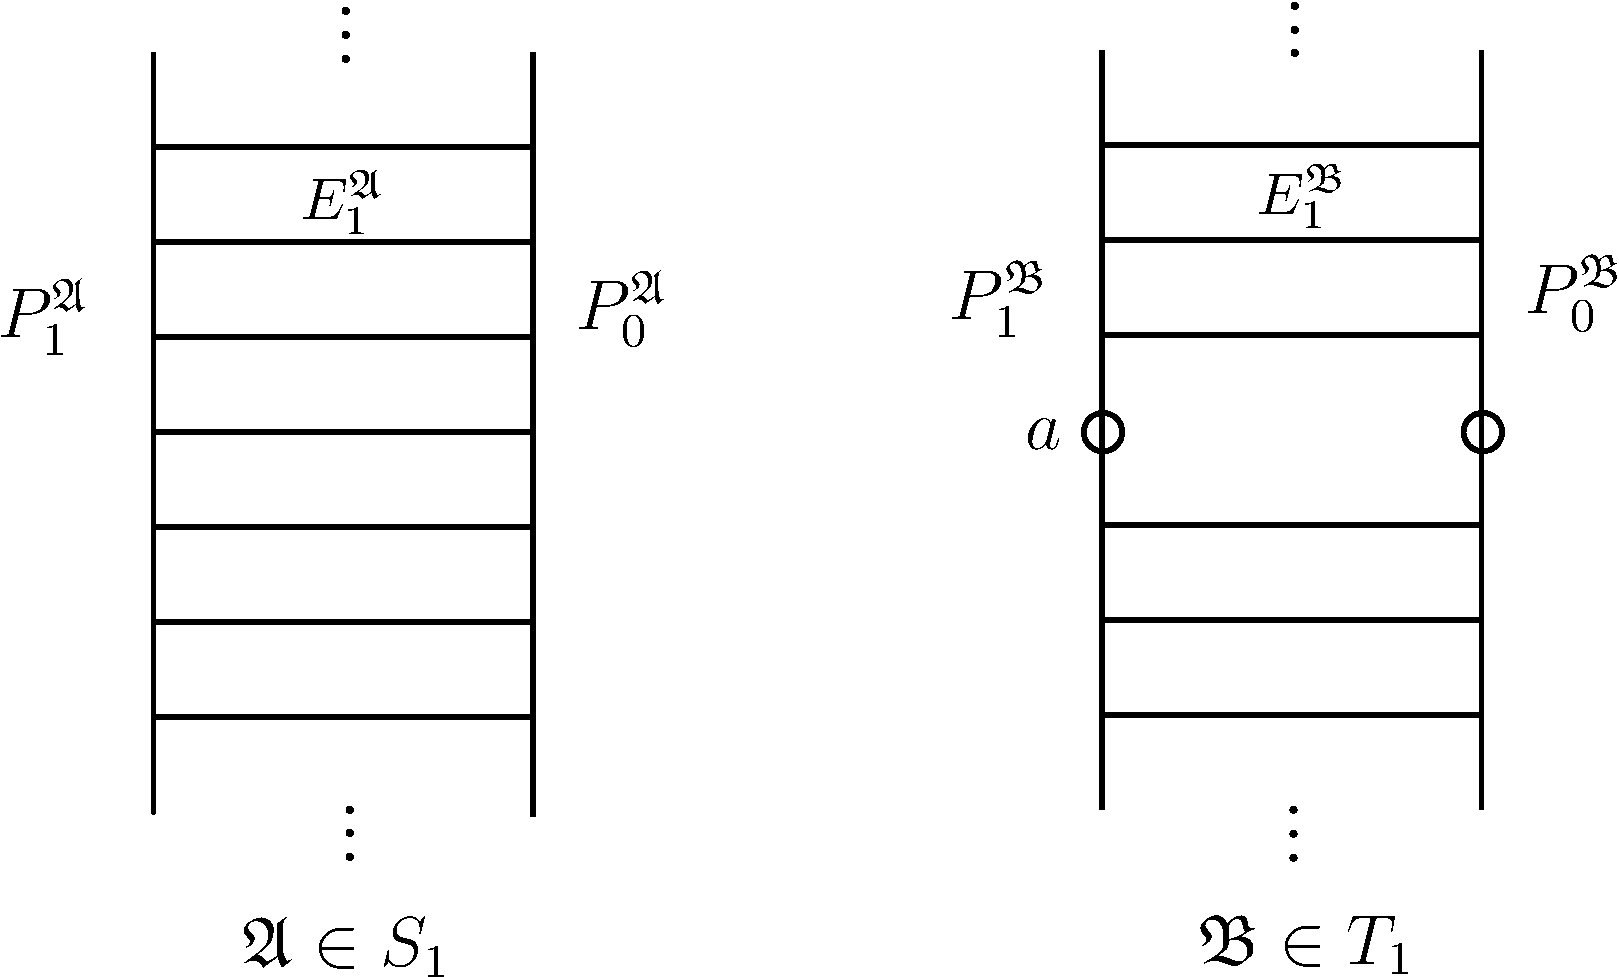
\includegraphics[scale = 0.4]{figs/figure1}
	\caption{Classes $S_1$ and $T_1$}
	\label{fig1}
\end{figure}

$\textbf{n > 1:}$ We define class $R_n \subset \Str[\tau_n]$ by setting $\mathfrak{A} \in R_n$ if and only if there is $\mathfrak{B} \in \Str[\{\leq\}]$ isomorphic to $\eta$ and structures $\mathfrak{M}_a \in \Str[\tau_{n-1}]$ for each $a \in B$ such that
\[
\mathfrak{A} \upharpoonright \tau_{n-1}  = \mathfrak{B} \cup \bigcup_{a \in B}\mathfrak{M}_a,
\]
$P_n^{\mathfrak{A}} = B$, and
\[
E_n^{\mathfrak{A}} = \{(x,y) \in A^2 \colon x \in P_n^{\mathfrak{A}} \text{ and } y \in M_x \}.
\]
Then we define classes $S_n$, $T_n$ by setting $\mathfrak{A} \in S_n$ if and only
if $\mathfrak{A} \in R_n$ and for all $a \in P_n^{\mathfrak{A}}$ we have
$\mathfrak{M}_a \in T_{n-1}$, and $\mathfrak{A} \in T_n$ if and only if there is
exactly one element $c \in P_n^{\mathfrak{A}}$ such that
$\mathfrak{M}_c \in S_{n-1}$ and $\mathfrak{M}_a \in T_{n-1}$ for all
$a \in P_n^{\mathfrak{A}} \setminus \{c\}$.
Figures \ref{fig1} and \ref{fig2} illustrate this construction.
For the remaining part of this text, we will write $\eta_n^{\mathfrak{A}}$ to
denote the structure $\mathfrak{B}$.
In addition, for each $a \in P^{\mathfrak{A}}_n$ we will write
$\mathfrak{M}^{\mathfrak{A}}_a$ to refer to the structure $\mathfrak{M}_a$.

\begin{figure}
	\centering
	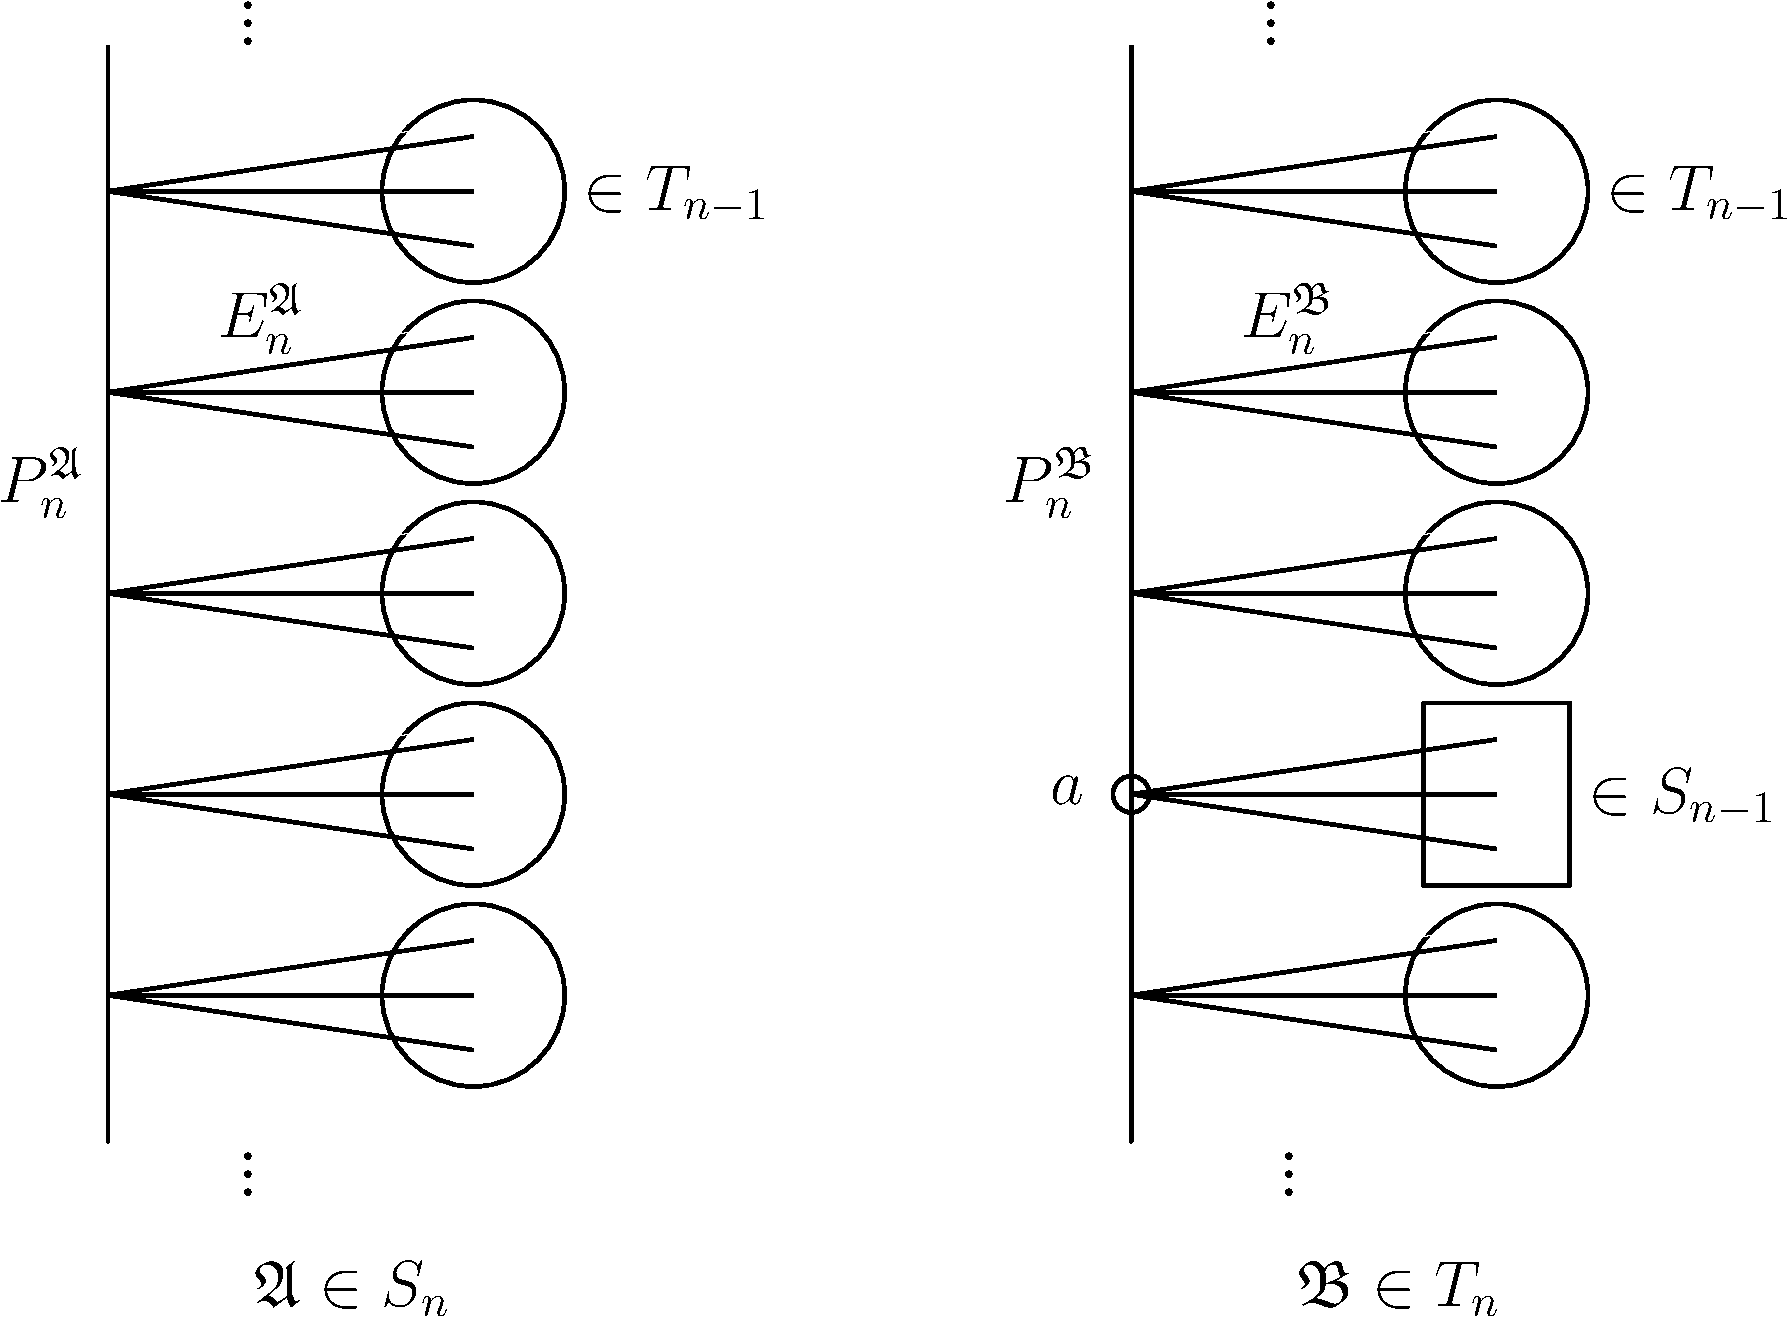
\includegraphics[scale = 0.4]{figs/figure2}
	\caption{Classes $S_n$ and $T_n$ for $n > 1$}
	\label{fig2}
\end{figure}

\end{construction}

\begin{lemma}\label{unique_struct}
Let $n\geq 1$ be a natural number.
Both $S_n$ and $T_n$ each have exactly one structure up to isomorphism.
\end{lemma}

\begin{proposition}\label{separation}
Suppose $n \geq 1$ is a natural number.
Let $\mathfrak{A} \in S_n$ and $\mathfrak{B} \in T_n$.
There is an $\mathcal{L}_{\omega\omega}[\tau_n]$-sentence $\varphi_n$ of
quantifier rank $n+1$ such that $\mathfrak{A} \vDash \varphi_n$ and
$\mathfrak{B} \nvDash \varphi_n$.
\end{proposition}
\begin{proof}
If $n = 1$, then we can set
$\varphi_1 = \forall x (P_1(x)\rightarrow \exists y (P_0(y) \wedge E_1(x,y)))$.
Thus, assume that $n > 1$ and such $\varphi_{n-1}$ exists.
Then we can set
\[
	\varphi_n = \forall x (P_n(x)\rightarrow \neg \varphi_{n-1}^{\{y \colon E_n(x,y)\}})
\]
where $\varphi_{n-1}^{\{y \colon E_n(x,y)\}}$ is the relativization of
$\varphi_{n-1}$ to the set $\{y \colon E_n(x,y)\}$.
\end{proof}

\begin{lemma}\label{right_emb}
Let $n \geq 1$ be a natural number and
$\mathfrak{A} \in S_n$, $\mathfrak{B}\in T_n$.
There is an embedding $f$ of $\mathfrak{A}$ into $\mathfrak{B}$ such that for
any $\overline{a} \in A^{<\omega}$ there are partitions $(A_1, A_2)$ of $A$ and
$(B_1, B_2)$ of $B$ such that
\begin{enumerate}
	\item $\overline{a} \in A_1^{<\omega}$,
	\item $f | A_1$ is an isomorphism between $\mathfrak{A} | A_1$ and $\mathfrak{B} | B_1$,
	\item $\mathfrak{A} | A_2 \cong \mathfrak{A}$ and $\mathfrak{B}|B_2 \cong \mathfrak{B}$,
	\item for every embedding
	$g \colon \mathfrak{A}|A_2\rightarrow \mathfrak{B}|B_2$ and
	$h \colon \mathfrak{B} |B_2 \rightarrow \mathfrak{A}|A_2$ it is the case that
	$(f|A_1) \cup g$ and $(f^{-1}|B_1) \cup h$ are embeddings
	$\mathfrak{A} \rightarrow \mathfrak{B}$ and
	$\mathfrak{B} \rightarrow \mathfrak{A}$, respectively,
	\item for any $m < \omega$, we have
	$(\mathfrak{A}, \overline{a}) \equiv^m_{\emb} (\mathfrak{B}, f\overline{a})$
	if and only if $\mathfrak{A} \equiv^m_{\emb} \mathfrak{B}$.
\end{enumerate}
\end{lemma}
\begin{proof}
We have two possible cases to consider: $n=1$ and $n > 1$.
First suppose that $n = 1$.
Let $a \in B$ be that unique element of $P_1^{\mathfrak{B}}$ for which there is
no $b \in B$ such that $(a, b) \in E_1^{\mathfrak{B}}$.
We use this element to define an ordering
$\xi_1 = \eta^{\mathfrak{B}}_1 | \{x \in B \colon x < a \}$.
It is easy to see by using Lemma \ref{order_isom} that there is an isomorphism
$h_1$ between $\eta^{\mathfrak{A}}_1$ and $\xi_1$.

Define function $f \colon A \rightarrow B$ by setting $f(x) = h_1(x)$ if
$x \in P_1^{\mathfrak{A}}$, and $f(x) = y$ if $x \in P^{\mathfrak{A}}_0$ where
$y \in P^{\mathfrak{B}}_0$ is such that there is $z \in P^{\mathfrak{A}}_1$ with
$\mathfrak{A} \vDash E_1(z,x)$ and $\mathfrak{B} \vDash E_1(h_1(z),y)$.
It is easy to see that $f$ is an embedding of $\mathfrak{A}$ into $\mathfrak{B}$.
Let $a_0,\dots,a_k \in A$. We must find partitions satisfying conditions 1-5.
For this, let $b, c \in A$ be such that
\begin{align*}
	\mathfrak{A} \vDash &P_1(b) \wedge P_0(c) \wedge E_1(b,c) \wedge \\
	&\bigwedge_{i\leq k}\big(\big(P_1(a_i) \rightarrow a_i<b\big) \wedge \big(P_0(a_i)\rightarrow a_i < c\big)\big).
\end{align*}
Now set $A_1 = \{x \in A \colon x \leq b \text{ or } x \leq c \}$, $B_1 = f[A_1]$,
and denote by $A_2$, $B_2$ the complements of $A_1$, $B_1$, respectively.
It is straightforward to verify that partitions $(A_1,A_2)$, $(B_1,B_2)$ satisfy
all the five requirements.
Notice that the fact 5 follows directly from the fact 4.
Thus, the case $n = 1$ is proved.

Assume now that $n > 1$.
By our construction, there is a unique element $a \in P_n^{\mathfrak{B}}$ such
that $\mathfrak{M}_a^{\mathfrak{B}} \in S_{n-1}$.
Define an ordering $\xi_n$ by setting
$\xi_n = \eta^{\mathfrak{B}}_n | \{x \in B \colon x < a \}$.
Again, as in the case $n = 1$, there is an isomorphism $h_n$ between
$\eta_n^{\mathfrak{A}}$ and $\xi_n$.

Thus, we have $\mathfrak{M}^{\mathfrak{A}}_x \in T_{n-1}$ for all
$x \in P^{\mathfrak{A}}_n$ and $\mathfrak{M}^{\mathfrak{B}}_x \in T_{n-1}$
for all $x \in \xi_n$ so, by Lemma \ref{unique_struct},
for each $x \in P_n^{\mathfrak{A}}$ there is an isomorphism $h_x$ between
$\mathfrak{M}^{\mathfrak{A}}_x$ and $\mathfrak{M}^{\mathfrak{B}}_{h(x)}$.
Then $f = h_n \cup \bigcup_{x\in P^{\mathfrak{A}}_n}h_x$ is a wanted embedding.
\end{proof}

\begin{lemma}\label{left_emb}
Let $n>1$ be a natural number and $\mathfrak{A} \in S_n$, $\mathfrak{B}\in T_n$.
There is an embedding $f$ of $\mathfrak{B}$ into $\mathfrak{A}$ such that for any
$\overline{a} \in B^{<\omega}$ there are partitions $(A_1,A_2)$ of $A$ and
$(B_1,B_2)$ of $B$ such that
\begin{enumerate}
	\item $\overline{a} \in B_1^{<\omega}$,
	\item $f | B_1$ is an isomorphism between $\mathfrak{B} | B_1$ and $\mathfrak{A} | A_1$,
	\item $\mathfrak{A}|A_2 \in T_{n-1}$ and $\mathfrak{B}|B_2 \in S_{n-1}$,
	\item for every embedding $g \colon \mathfrak{A}|A_2\rightarrow \mathfrak{B}|B_2$
	and $h \colon \mathfrak{B}' |B_2\rightarrow \mathfrak{A}'|A_2$ it is the case
	that $(f^{-1}|A_1) \cup g$ and $(f|B_1) \cup h$ are embeddings
	$\mathfrak{A} \rightarrow \mathfrak{B}$ and
	$\mathfrak{B} \rightarrow \mathfrak{A}$, respectively,
	\item we have
	$(\mathfrak{A}, f\overline{a}) \equiv^{n-1}_{\emb} (\mathfrak{B}, \overline{a})$
	if and only if $\mathfrak{M} \equiv^{n-1}_{\emb} \mathfrak{N}$ for all
	$\mathfrak{M} \in T_{n-1}$ and $\mathfrak{N} \in S_{n-1}$.
\end{enumerate}
\end{lemma}
\begin{proof}
Let $h$ be an isomorphism between $\eta^{\mathfrak{B}}_n$ and
$\eta^{\mathfrak{A}}_n$, and let $a \in P_n^{\mathfrak{B}}$ be the unique
element for which $\mathfrak{M}_a^{\mathfrak{B}} \in S_{n-1}$.
For each $x \in P_n^{\mathfrak{B}} \setminus \{a\}$ let $h_x$ be an isomorphism
between $\mathfrak{M}^{\mathfrak{B}}_x$ and $\mathfrak{M}^{\mathfrak{A}}_{h(x)}$,
and let $h_a$ be an embedding of $\mathfrak{M}^{\mathfrak{B}}_a$ into
$\mathfrak{M}^{\mathfrak{A}}_{h(a)}$ as given by Lemma \ref{right_emb}.

Let $f = h \cup \bigcup_{x\in P^{\mathfrak{B}}_n}h_x$.
Then $f$ is an embedding of $\mathfrak{B}$ into $\mathfrak{A}$.
Note that $\mathfrak{M}^{\mathfrak{B}}_a \in S_{n-1}$ and
$\mathfrak{M}^{\mathfrak{A}}_{h(a)} \in T_{n-1}$, and for all embeddings
$g \colon \mathfrak{M}^{\mathfrak{B}}_a \rightarrow \mathfrak{M}^{\mathfrak{A}}_{h(a)}$ and
$g' \colon \mathfrak{M}^{\mathfrak{A}}_{h(a)} \rightarrow \mathfrak{M}^{\mathfrak{B}}_a$
the functions $f' \cup g$ and $f'^{-1} \cup g'$ are also embeddings
$\mathfrak{B} \rightarrow \mathfrak{A}$ and $\mathfrak{A} \rightarrow \mathfrak{B}$,
respectively, where
$f' = h\cup \bigcup_{x\in P_n^{\mathfrak{B}}\setminus \{a\}} h_x$.

Let $\overline{a} \in B^{<\omega}$, $\overline{a} = (a_1,\dots,a_k)$, and assume
without loss of generality that $a_1,\dots,a_m \in B\setminus M_a$ and
$a_{m+1},\dots,a_k \in M_a$ for some $m\leq k$.
In what follows we will write $\mathfrak{M}_x$ instead of
$\mathfrak{M}_x^{\mathfrak{A}}$ or $\mathfrak{M}_x^{\mathfrak{B}}$.
By Lemma \ref{right_emb}, there are partitions $(M_1,M_2)$ of $M_a$ and
$(N_1,N_2)$ of $M_{h(a)}$ such that
\begin{enumerate}
	\item $a_{m+1},\dots,a_k \in M_1$,
	\item $h_a|M_1$ is an isomorphism between $\mathfrak{M}_a | M_1$ and
	$\mathfrak{M}_{h(a)} | N_1$,
	\item $\mathfrak{M}_a | M_2 \in S_{n-1}$ and
	$\mathfrak{M}_{h(a)} | N_2 \in T_{n-1}$,
	\item for every embedding
	$g \colon \mathfrak{M}_a|M_2 \rightarrow \mathfrak{M}_{h(a)}|N_2$ and
	$g' \colon \mathfrak{M}_{h(a)}|N_2 \rightarrow \mathfrak{M}_a | M_2$ we have that
	$(h_a | M_1) \cup g$ and $(h_a^{-1} | N_1)\cup g'$ are also embeddings
	$\mathfrak{M}_a \rightarrow \mathfrak{M}_{h(a)}$ and
	$\mathfrak{M}_{h(a)} \rightarrow \mathfrak{M}_a$, respectively.
\end{enumerate}
Now let $A_1 = A \setminus N_2$, $A_2 = N_2$, $B_1 = B \setminus M_2$ and $B_2 = M_2$.
Then $(A_1,A_2)$ and $(B_1,B_2)$ are partitions of $A$ and $B$, respectively,
satisfying all the five requirements.
\end{proof}

\begin{lemma}\label{one_equiv}
Let $\mathfrak{A} \in S_1$ and $\mathfrak{B} \in T_1$.
Then $\mathfrak{A} \equiv_{\emb}^1 \mathfrak{B}$.
\end{lemma}
\begin{proof}
We already proved that there is an embedding of $\mathfrak{A}$ into $\mathfrak{B}$
in Lemma \ref{right_emb}, so we only need to find an embedding of $\mathfrak{B}$
into $\mathfrak{A}$.
We expand the vocabulary $\tau_1$ by setting
$\tau^*_1 = \tau_1 \cup \{c_q,d_q \colon q \text{ is a rational number } \}$
where all $c_q$, $d_q$ are distinct constant symbols.
Let $h \colon \eta \rightarrow \eta^{\mathfrak{A}}_1$ and
$g \colon \eta \rightarrow \eta^{\mathfrak{B}}_1$ be isomorphisms.
Let $a \in \eta$ be that unique element for which there is no
$b \in \eta_0^{\mathfrak{B}}$ such that $\mathfrak{B} \vDash E_1(g(a), b)$.

Let $\mathfrak{A}^*$, $\mathfrak{B}^*$ be $\tau^*$-structures such that
$\mathfrak{A}^* \upharpoonright \tau_1 = \mathfrak{A}$ and
$\mathfrak{B}^*\upharpoonright \tau_1 = \mathfrak{B}$,
$c^{\mathfrak{A}^*}_q = h(q)$, $c^{\mathfrak{B}^*}_q = g(q)$ for all $q\in \eta$,
$d_q^{\mathfrak{A}^*}$, $d_q^{\mathfrak{B}^*}$ are such that
$\mathfrak{A}^* \vDash E_1(c_q, d_q)$ for all $q \in \eta$ and
$\mathfrak{B}^* \vDash E_1(c_q, d_q)$ for all $q \in \eta \setminus \{a\}$,
and $d_a^{\mathfrak{B}^*}$ is that element $z$ of $\eta_0^{\mathfrak{B}}$
for which there is no element $y \in \eta_1^{\mathfrak{B}}$ such that
$\mathfrak{B} \vDash E_1(y, z)$.
We define a function $f \colon B \rightarrow A$ by setting
\begin{align*}
	&\left. \begin{array}{rl}
	f(c_q^{\mathfrak{B}^*}) = c_{q+1}^{\mathfrak{A}^*}, \\
	f(d_q^{\mathfrak{B}^*}) = d_{q+1}^{\mathfrak{A}^*} \\
	\end{array} \right\} \text{ if } q > a, \\
	&\left. \begin{array}{rl}
	f(c_q^{\mathfrak{B}^*}) = c_{q-1}^{\mathfrak{A}^*}, \\
	f(d_q^{\mathfrak{B}^*}) = d_{q-1}^{\mathfrak{A}^*} \\
	\end{array} \right\} \text{ if } q < a,\\
	&\ \ f(c^{\mathfrak{B}^*}_a) = c^{\mathfrak{A}^*}_a, \\
	&\ \ f(d^{\mathfrak{B}^*}_a) = d^{\mathfrak{A}^*}_{a+\frac{1}{2}}.
\end{align*}
It is straightforward to verify that $f$ is indeed an embedding of
$\mathfrak{B}$ into $\mathfrak{A}$.
\end{proof}

\begin{proposition}\label{n_equiv}
Let $n \geq 1$ be a natural number and $\mathfrak{A}\in S_n$,
$\mathfrak{B}\in T_n$.
Then $\mathfrak{A} \equiv_{\emb}^n \mathfrak{B}$.
\end{proposition}
\begin{proof}
We use induction on $n$. The base case is proved in Lemma \ref{one_equiv}.
Assume that $n>1$ and the claim is true for $n-1$.
Let Duplicator select embeddings $f \colon \mathfrak{A} \rightarrow \mathfrak{B}$
as in Lemma \ref{right_emb} and $g \colon \mathfrak{B} \rightarrow \mathfrak{A}$
as in Lemma \ref{left_emb}.
Suppose first that Spoiler chose embedding $f$ and elements $a_1,\dots,a_k \in A$.
Let $(A_1,A_2)$ and $(B_1,B_2)$ be partitions of $A$ and $B$, respectively,
as given by Lemma \ref{right_emb}.
Then $(\mathfrak{A},\overline{a}) \equiv^{n-1}_{\emb} (\mathfrak{B},f\overline{a})$
by the fact 5. of Lemma \ref{right_emb} and the induction hypothesis.
Now suppose that Spoiler selected the embedding $g$ and elements $b_1,\dots,b_l \in B$.
Let $(A^*_1,A^*_2)$ and $(B^*_1,B^*_2)$ be partitions of $A$ and $B$, respectively,
as given by Lemma \ref{left_emb}.
Then by its 5. fact we have
$(\mathfrak{A},g\overline{b}) \equiv^{n-1}_{\emb} (\mathfrak{B},\overline{b})$.
Thus, since also
$(\mathfrak{A},\overline{a}) \equiv^{n-1}_{\emb} (\mathfrak{B},f\overline{a})$,
we have $\mathfrak{A} \equiv^n_{\emb} \mathfrak{B}$.
\end{proof}

\begin{proof}[Proof of Theorem \ref{main}]
Combine Propositions \ref{separation} and \ref{n_equiv}.
The existence of $\varphi_n$ having the required form with alternating existence
and universal quantifiers follows from the proof of Proposition \ref{separation}.
\end{proof}

\begin{remark}
In the proof of Theorem \ref{main} we used a tree construction in which new
structures were built from given structures by connecting them in a specific way.
This sort of construction is often encountered in proofs of  undefinability results.
For example, a result similar to Theorem \ref{main} concerning logics with
quantifiers of bounded arity was proved in \cite{Keisler:2011} by Keisler and
Lotfallah.
They used an analogous tree construction and the bijective game
(see Remark \ref{bijective}) in their proof.
Worth mentioning are also tree-like sums of Makowsky and Shelah in
\cite{Makowski:1979} based on ideas of Friedman \cite{Friedman:1973} and
Gregory \cite{Gregory:1974}.
They are used to prove some results concerning, among others, Beth definability
in abstract logics.
\end{remark}

\bibliographystyle{jflnat}
\bibliography{refs2}

\end{document}
